% Keep Wiley's supplied class and support files in their own directory while
% making that directory available to package lookups performed by USG.cls.
\makeatletter
\def\input@path{{latex/wiley/}}
\makeatother
\documentclass[ASNA]{latex/wiley/USG}

% Retain the supplied class for the manuscript body, but use a deliberately
% plain author-manuscript front matter with no journal branding or publication
% metadata. The additional packages support manuscript tables, supplementary
% landscape pages, and the blue revision markup.
\usepackage{anyfontsize}
\usepackage{fontspec}
\setmainfont{STIX-Regular.otf}[
  Path=latex/wiley/Fonts/Stix/,
  BoldFont=STIX-Bold.otf,
  ItalicFont=STIX-Italic.otf,
  BoldItalicFont=STIX-BoldItalic.otf
]
\usepackage{colortbl}
\usepackage{xcolor}
\usepackage{longtable}
\newcounter{none}
\renewcommand{\thenone}{}
\usepackage{pdflscape}
\usepackage{caption}
\usepackage{hanging}
\usepackage[section]{placeins}

\graphicspath{{FlowMOP_submission_media/}{figs_data/}}

\definecolor{revisionblue}{HTML}{0066CC}
\providecommand{\tightlist}{\setlength{\itemsep}{0pt}\setlength{\parskip}{0pt}}
\providecommand{\pandocbounded}[1]{#1}
\providecommand{\passthrough}[1]{#1}


\begin{document}

\pagestyle{plain}
\floatpagestyle{plain}
\rotfloatpagestyle{plain}
\setlength{\parindent}{0pt}
\setlength{\parskip}{\baselineskip}

\begin{center}
{\LARGE\bfseries FlowMOP: An Automated Flow Cytometry Time, Debris, and
Doublet Removal Tool\par}
\vspace{1em}
{\normalsize
Tony Xu\textsuperscript{1},
Nadia A. Roberts\textsuperscript{1},
Felix Marsh-Wakefield\textsuperscript{2,3},
Rebecca A. Jaeger\textsuperscript{1},
Sarah Croft\textsuperscript{1},
Abhimanu Pandey\textsuperscript{1},
Dalton Leibold\textsuperscript{4},
Angela L. Ferguson\textsuperscript{2,3},
Lily Rodgers\textsuperscript{2,3},
Umaimainthan Palendira\textsuperscript{3},
Geoffrey W. McCaughan\textsuperscript{2,5,6},
Ben Quah\textsuperscript{7},
Robin Vlieger\textsuperscript{8,*}, and
Anne Brüstle\textsuperscript{1,*}\par}
\vspace{0.8em}
{\small
\textsuperscript{1}Department of Immunology and Infectious Disease, John Curtin School of Medical Research, The Australian National University, Canberra, Australian Capital Territory, Australia\par
\textsuperscript{2}Liver Injury \& Cancer Program, Cancer Innovations Centre, Centenary Institute, The University of Sydney, Sydney, New South Wales, Australia\par
\textsuperscript{3}Human Immunology Laboratory, School of Medical Sciences, Faculty of Medicine and Health, The University of Sydney, Sydney, New South Wales, Australia\par
\textsuperscript{4}Division of Ecology and Evolution, Research School of Biology, The Australian National University, Canberra, Australian Capital Territory, Australia\par
\textsuperscript{5}A.W. Morrow Gastroenterology and Liver Centre, Royal Prince Alfred Hospital, Sydney, New South Wales, Australia\par
\textsuperscript{6}Sydney Medical School, Faculty of Medicine and Health, The University of Sydney, Sydney, New South Wales, Australia\par
\textsuperscript{7}Division of Genome Sciences and Cancer, John Curtin School of Medical Research, The Australian National University, Canberra, Australian Capital Territory, Australia\par
\textsuperscript{8}School of Medicine and Psychology, The Australian National University, Canberra, Australian Capital Territory, Australia\par}
\end{center}

\noindent\textbf{Correspondence:} Robin Vlieger (\href{mailto:Robin.Vlieger@anu.edu.au}{Robin.Vlieger@anu.edu.au}) and Anne Brüstle (\href{mailto:Anne.Bruestle@anu.edu.au}{Anne.Bruestle@anu.edu.au})

\par\noindent\textbf{Funding:} TX is supported by the Australian
Government Research Training Program PhD Scholarship. There are no other
relevant sources of funding.

\section*{Abstract}
Flow cytometry now generates high-parameter datasets whose scale and
variability challenge manual preprocessing, leading to subjectivity and
poor reproducibility. Temporal artifacts are acquisition-time-dependent
deviations in event quality or fluorescence signal caused by blockages,
bubbles, flow instability, or instrument instability. This study
introduces FlowMOP, a Python-native framework that automates three major
preprocessing steps---time-gating, debris removal, and doublet
exclusion. FlowMOP was developed to combine these preprocessing steps in
a single workflow, whereas FlowCut and PeacoQC primarily address
time-dependent quality control and broader automatic gating frameworks
are aimed at population identification rather than standardized
preprocessing cleanup.

Methodologically, temporal artifacts are identified via parameter-wise
peak checks, bin-level fluorescence summaries across acquisition time,
and robust outlier rejection. Debris is excluded by adaptive FSC-A
thresholding derived from cross-parameter peak structure. Finally,
doublets are removed using dynamic inflection detection on FSC-A/FSC-H
and SSC-A/SSC-H ratio histograms. The implementation uses
memory-conscious array operations; computational scaling was evaluated
to 2 million events in a 36-channel file.

Validation used synthetic datasets with event-level ground truth for
acquisition-time artifacts, debris enrichment, and doublet enrichment,
together with an exploratory expert comparison on biological datasets.
In the synthetic time-gating benchmark, FlowMOP had higher sensitivity
than FlowCut for Segment artifacts at both tested bin sizes and in the
5000-event Bimix and Trimix settings, and higher specificity than both
competitors across all three 5000-event scenarios. FlowMOP also removed
labelled debris and doublet populations effectively in technical-control
datasets. The expert comparison, which used an earlier FlowMOP
configuration, generally favoured manual gates and is reported in the
Supplementary Information. \textbf{{[}PLACEHOLDER: Principal
biological-validation finding from Figure 5.{]}} \textbf{{[}PLACEHOLDER:
Principal tumour-validation finding from Figure 6.{]}} Within the tested
settings, FlowMOP provides a reproducible workflow for standardizing
time, debris, and doublet preprocessing. FlowMOP can be accessed at
\url{https://github.com/1ordinateur/FlowMOP}.

\section*{Contact information for all authors}
Tony Xu
\href{mailto:Tony.Xu@anu.edu.au}{\nolinkurl{Tony.Xu@anu.edu.au}}; Nadia
A. Roberts
\href{mailto:Nadia.Roberts@anu.edu.au}{\nolinkurl{Nadia.Roberts@anu.edu.au}};
Felix Marsh-Wakefield
\href{mailto:felix.marsh-wakefield@sydney.edu.au}{\nolinkurl{felix.marsh-wakefield@sydney.edu.au}};
Rebecca A. Jaeger
\href{mailto:Rebecca.Jaeger@anu.edu.au}{\nolinkurl{Rebecca.Jaeger@anu.edu.au}};
Sarah Croft
\href{mailto:Sarah.Croft@anu.edu.au}{\nolinkurl{Sarah.Croft@anu.edu.au}};
Abhimanu Pandey
\href{mailto:Abhimanu.Pandey@anu.edu.au}{\nolinkurl{Abhimanu.Pandey@anu.edu.au}};
Dalton Leibold
\href{mailto:Dalton.Leibold@anu.edu.au}{\nolinkurl{Dalton.Leibold@anu.edu.au}};
Angela L. Ferguson
\href{mailto:a.ferguson@centenary.org.au}{\nolinkurl{a.ferguson@centenary.org.au}};
Lily Rodgers
\href{mailto:lrod8310@uni.sydney.edu.au}{\nolinkurl{lrod8310@uni.sydney.edu.au}};
Umaimainthan Palendira
\href{mailto:umaimainthan.palendira@sydney.edu.au}{\nolinkurl{umaimainthan.palendira@sydney.edu.au}};
Geoffrey W. McCaughan
\href{mailto:g.mccaughan@centenary.org.au}{\nolinkurl{g.mccaughan@centenary.org.au}};
Ben Quah
\href{mailto:ben.quah@anu.edu.au}{\nolinkurl{ben.quah@anu.edu.au}};
Robin Vlieger
\href{mailto:Robin.Vlieger@anu.edu.au}{\nolinkurl{Robin.Vlieger@anu.edu.au}};
Anne Brüstle
\href{mailto:Anne.Bruestle@anu.edu.au}{\nolinkurl{Anne.Bruestle@anu.edu.au}}

\section*{Acknowledgements}
We thank Givanna Putri for her very helpful feedback and suggestions
throughout the manuscript's preparation. This work was also supported by
computational resources provided by the Australian Government through
the National Computational Infrastructure (NCI) under the ANU Merit
Allocation Scheme.

\FloatBarrier

\section{Introduction}\label{introduction}

Modern flow-cytometry studies can contain increasing numbers of files,
events, and measured parameters {[}2{]}. The large scale of these data
makes repeated manual preprocessing time-consuming and often
impractical, potentially amplifying variability between operators.
Reproducible automated preprocessing is therefore valuable for large
studies.

Manual preprocessing of flow cytometry data, whilst still not
standardised, typically involves three gating components. I) Time
gating: operators perform time-gating to remove events potentially
acquired erroneously due to transient or persistent artifacts in the
instrument or sample, including air bubbles, blockages, or laser
malfunctions. II) Debris gating: operators remove debris, which is
generated by both the sample preparation process and inherent in the
sample itself. Debris events are generally identified by reference to
measured events with low size (determined by FSC-A (Forward SCatter --
Area)) and internal complexity (determined by SSC-A (Side SCatter --
Area)) {[}1{]}. III) Doublet gating: Events classified as
"doublets"---two or more cells erroneously detected as one---are removed
as their fluorescence measurements lack reliability. This is often done
with reference to the ratio of the signal duration, and signal
intensity. Doublets feature a signal peak strength comparable to a
single cell, but for twice the duration. Hence, analysts may filter
these events out by comparing an event's total FSC Area relative to its
FSC height (peak signal intensity) or by comparing the FSC signal height
against the FSC signal width {[}4{]}. These manual preprocessing steps
are time-consuming, inherently subjective, and susceptible to
inconsistency across operators.

The most conspicuous time artifacts often occur at the beginning or end
of acquisition, but flow-rate surges interspersed throughout acquisition
and associated signal-intensity variation have also been documented
{[}10{]}. Here, we use ``microblockage'' operationally to denote a
short, self-resolving mid-acquisition disturbance that produces a
localized fluorescence shift; the term does not imply that a physical
obstruction was directly observed. Temporary acquisition problems can be
difficult to detect manually {[}5{]}, and manual identification and
removal of transient problems can be time-consuming and subjective
{[}9{]}. Because the affected intervals may be short and interspersed
with otherwise plausible events, they can be impractical to exclude
reproducibly using multiple manual gates.

Several tools automate cytometry population identification, including
the model-based flowClust method {[}13{]}, the neural-network method
GateNet {[}14{]}, and the bivariate-segmentation framework UNITO
{[}15{]}; automated gating approaches are reviewed elsewhere {[}16{]}.
FlowMOP is a Python-based, training-free preprocessing workflow that
combines automated time-gating, debris removal, and doublet exclusion in
a single headless tool. FlowCut and PeacoQC provide the most direct
comparison for its time-gating component.

The Python implementation specifically facilitates integration with
contemporary machine-learning workflows, which predominantly utilize
Python-based frameworks.

To date, cytometry preprocessing algorithms have been evaluated either
by comparison to human-defined gold standards (as in FlowCut and
PeacoQC) or through mathematical metrics (consider cyCombine's approach
to batch correction {[}11{]}). The synthetic datasets provide
event-level labels for estimating sensitivity and specificity in
preprocessing tasks where real ground truth is otherwise difficult to
define.

Here, we introduce FlowMOP, an automated preprocessing tool for
time-gating, debris removal, and doublet exclusion. We compare
time-gating performance with PeacoQC and FlowCut, evaluate debris and
doublet removal using synthetic ground-truth datasets and expert
comparison, and benchmark computational scalability.

\FloatBarrier

\section{Methods}\label{methods}

For further details concerning datasets, see Supplementary Table 1A.

\subsection{Preparation protocols for synthetic
samples}\label{preparation-protocols-for-synthetic-samples}

\subsubsection{Synthetic Time Sample Preparation and
Generation}\label{synthetic-time-sample-preparation-and-generation}

\subsubsection{Preparation of Human PBMC Samples for Synthetic Time
Benchmarking
Samples}\label{preparation-of-human-pbmc-samples-for-synthetic-time-benchmarking-samples}

PBMC samples were collected from healthy donors under ethics protocols
ACT Health 2019.ETH.00081 and ANU HREC 2020/047. Blood was collected
into ACD-A tubes and PBMCs isolated using Lymphoprep density gradient
(Stemcell Technologies) and SepMate tubes (Stemcell Technologies) per
manufacturer's instructions prior to cryopreservation. Thawed PBMCs were
stained with ViaDye Red (Cytek Biosciences). The staining cocktail
contained antibodies to several highly abundant antigens at
less-than-saturating concentrations, and either 0.5, 1 or 3 x 10\^{}6
cells were stained, yielding samples with different levels of
fluorophore signal intensity for these common antigens. Other antibodies
within the panel were present at saturating concentrations to yield
similar fluorescence intensity across different cell seeding densities.
Samples were acquired on a Cytek Northern Lights 3-laser (V/B/R)
spectral flow cytometer.

\subsubsection{Generation of Synthetic Time
Samples}\label{generation-of-synthetic-time-samples}

Samples were synthetically combined across differing cell concentrations
in three manners. Their construction is shown in Figure S1. One in a
simple `Segmented' fashion, where events from one or more samples were
simply appended onto events from an existing sample. The second, `Bimix'
manner, where events from two differently stained samples were randomly
synthetically combined in random proportions (e.g. 40:60, 75:25 etc),
with one run containing a mixing bin size of 5000 events and the other
of 2000 events. The final, `Trimix' contained randomly combined events
from three differently stained samples in mixing bin sizes of 5000, and
2000 events. Here, we use ``microblockage'' operationally to denote a
short, self-resolving mid-acquisition disturbance that produces a
localized fluorescence shift; the term does not imply that a physical
obstruction was directly observed. Segmented samples model sustained
changes, whereas Bimix and Trimix model the observable fluorescence
consequence in this operational definition by introducing short
source-defined fluorescence shifts during acquisition. They do not
recreate or establish the physical mechanism itself. The Bimix and
Trimix files can appear acceptable on visual inspection because the
altered intervals are short and interspersed with otherwise plausible
events; however, the retained source labels identify the intentionally
perturbed events that should be excluded under the benchmark definition.
This provides event-level ground truth for a class of artifact that is
difficult to recognize and impractical to gate manually {[}5,9{]}.
Flow-rate disturbances without corresponding fluorescence changes should
not prompt event exclusion; these samples therefore model fluorescence
changes across acquisition order without introducing flow-rate
disturbances. Flow-rate effects were tested separately by altering Time
either in alignment with source-linked fluorescence changes or
independently of them.

\subsubsection{Time-only acquisition-rate mechanism
benchmark}\label{time-only-acquisition-rate-mechanism-benchmark}

To distinguish acquisition-rate sensitivity from source-linked
fluorescence and composition structure, we performed a matched mechanism
benchmark using source-labelled smallcut synthetic-combo FCS files.
Thirty high-count inputs were selected: ten Bimix, ten Trimix, and ten
Segment files. For each file, 500,000 acquisition-order-preserving
events were used without changing fluorescence, scatter, source labels,
or event order. Bimix and Trimix files used the first 500,000 events;
Segment files used a contiguous 500,000-event window centered on the
source transition so that both segment sources were represented.

Each input generated three matched variants: raw, source-time-warped,
and random-time-warped. In the source-time-warped variant, local Time
increments were multiplied according to source identity using
acquisition-interval multipliers spanning 1.0x to 20.0x. In the
random-time-warped variant, the same multiplier range was assigned to
contiguous 25,000-event chunks independently of source identity. After
warping, the total Time range was rescaled to match the raw input so
that the benchmark tested local acquisition-rate structure rather than
total acquisition duration. FlowMOP, FlowCut, and PeacoQC were run on
each matched input. Performance was evaluated relative to the matched
raw file using sensitivity and specificity.

\subsubsection{MAD-smoothing ablation and default
selection}\label{mad-smoothing-ablation-and-default-selection}

To test spline smoothing directly, FlowMOP was rerun across all 173
primary synthetic time-gating inputs with all non-smoothing settings
fixed. Nineteen short/long smoothing-factor pairs, including a
no-smoothing control, were compared by equally weighting the six
benchmark groups. The current default (\texttt{0.01,0.05}) was selected
as the marginally highest-scoring smoothed setting on this balanced
comparison (Table S4). Figure 2 was regenerated using this setting. All
completed quantitative FlowMOP results retained in the main figures use
the current selected configuration for the relevant module, and the
planned biological-validation figures will likewise use the current
configuration. The earlier expert preference evaluation used a previous
FlowMOP configuration; because updating it would require repeating the
blinded expert assessment, it is presented as an exploratory
supplementary analysis (Figs. S5-S7).

\subsubsection{Mice}\label{mice}

For generation of synthetic samples for FlowMOP validation (debris and
doublet removal), splenocytes from 13-16-week old C57Bl/6N or C57Bl/6J
mice were used. All animal experimentation was performed under ethics
protocol 2024/379 at the Australian Phenomics Facility at the Australian
National University, Canberra.

\subsubsection{Synthetic Debris Sample Preparation and
Generation}\label{synthetic-debris-sample-preparation-and-generation}

Mouse spleens were mechanically dissociated prior to lysis of red blood
cells (RBC) with RBC lysis buffer (MilliQ H2O containing 150 mM NH4Cl,
10 mM KHCO3 and 1 mM EDTA). Splenocytes were then incubated with Fc
block (BD), then stained with an antibody panel to delineate several
major immune cell subsets (CD19 APC, CD3 PE, CD8 PE-Cy7, CD11b BB515,
CD4 BV605, Fixable Viability Dye efluor780). To generate `high debris'
samples, cells were resuspended in MilliQ water and incubated for 2
minutes, prior to addition of 10X PBS to restore osmolarity. `Low
debris' samples were kept in isotonic solution throughout. Samples were
acquired using a BD LSRII cytometer.

For assessment of FlowMOP debris-gating performance, high-debris and
low-debris samples were combined by sampling approximately equal event
numbers from each source and concatenating them into matched synthetic
mixtures while retaining source labels for ground-truth quantification.

\subsubsection{Synthetic Doublet Sample Preparation and
Generation}\label{synthetic-doublet-sample-preparation-and-generation}

To generate samples with high proportions of doublets, mouse spleens
were digested through injection with digestion buffer comprising RPMI
(Gibco) supplemented with collagenase P (Roche) and DNAse I (Roche).
After incubation and mechanical dissociation, red blood cells (RBCs)
were lysed with RBC lysis buffer. Cells were then divided and stained
with either CellTrace Violet (CTV) (Invitrogen) or Carboxyfluorescein
succinimidyl ester (CFSE) (eBioscience). Following this, cells were
recombined and incubated for 30 minutes at 37oC 5\% CO2 to encourage
further doublet formation, then stained with Fixable Viability Dye
eFluor780 (Invitrogen). Samples were acquired on a BD LSRII cytometer.

\subsection{Non-synthetic samples}\label{non-synthetic-samples}

Human liver samples used in the non-synthetic validation datasets were
collected under ethics approval from the Sydney Local Health District
Ethics Review Committee (X19-0488 and 2019/ETH13790).

\subsection{Biological-validation
analysis}\label{biological-validation-analysis}

\textbf{{[}PLACEHOLDER: Figure 5 biological-validation samples,
preprocessing comparisons, prespecified biological endpoints, and
statistical analysis.{]}}

\subsection{Tumour-liver acquisition-instability and
biological-concordance
analysis}\label{tumour-liver-acquisition-instability-and-biological-concordance-analysis}

\textbf{{[}PLACEHOLDER: Update this section to match
Felix\textquotesingle s final Figure 6 tumour-validation analysis.{]}}

Three tumour and three non-tumour human liver FCS files were used for an
additional biological validation. For the acquisition-instability
analysis, the three tumour files were divided into common
acquisition-order bins, and the time masks produced by manual gating,
FlowMOP, FlowCut, and PeacoQC were projected onto those bins. Bin-level
deviations were evaluated using fluorescence channels only; Time, FSC,
and SSC measurements were excluded. Method-overlap and method-specific
residual bins were then examined using robustly scaled fluorescence
summaries and positive-population deviations.

For the downstream analysis, the FlowMOP output was defined as the
intersection of its independently calculated time, debris, and doublet
masks; the limit-of-detection mask was excluded. The corresponding
manual population was reconstructed from the final time, cells, and
single-cell gates in the FlowJo workspace. Zombie-low events were
defined operationally as Zombie UV-A values below 12,000 raw units, with
the same threshold applied to every sample. This threshold-based
analysis was used as an orthogonal biological-concordance check and not
as a universal live/dead classifier.

To separate selective Zombie-high exclusion from the overall extent of
event removal, selectivity was defined within each sample as the
Zombie-high removal rate divided by the Zombie-low removal rate. The
primary comparison was the paired FlowMOP/manual selectivity
fold-change. Because selectivity is multiplicative and the sample size
was small, FlowMOP and manual values were compared using an exact
two-sided Wilcoxon signed-rank test applied to the log-transformed
paired ratios. Constituent time, debris, and doublet masks were
evaluated separately as secondary mechanistic analyses. No equivalence
or non-inferiority margin was prespecified; consequently, a
non-significant paired comparison was interpreted as no detected
difference rather than proof of equivalence.

\subsection{Computational scalability
benchmark}\label{computational-scalability-benchmark}

Computational scalability was evaluated using clone-based real-FCS
scaling. A representative FCS file was subsampled/replicated to matched
event counts of 10,000, 100,000, 300,000, 1,000,000, and 2,000,000
events while preserving the original 36-channel structure. FlowMOP,
PeacoQC, and FlowCut were run on the same generated inputs for each
size.

For fair timing of the shared time-gating task, FlowMOP was run using
local non-distributed execution, with debris and doublet removal
disabled and annotated output FCS writing disabled. PeacoQC and FlowCut
were run with optional plotting, reporting, and output generation
disabled where supported. Each condition was run once as a warm-up and
then three measured times. Runtime and peak resident memory were
recorded using \texttt{/usr/bin/time\ -v}; means and standard deviations
were calculated across the three measured repeats.

\subsection{Coding Assistance}\label{coding-assistance}

Parts of the code were generated with the aid of ChatGPT Codex and
Claude Code. All code generated by LLMs were manually verified before
implementation.

\FloatBarrier

\section{RESULTS}\label{results}

\begin{figure}[p]
\centering
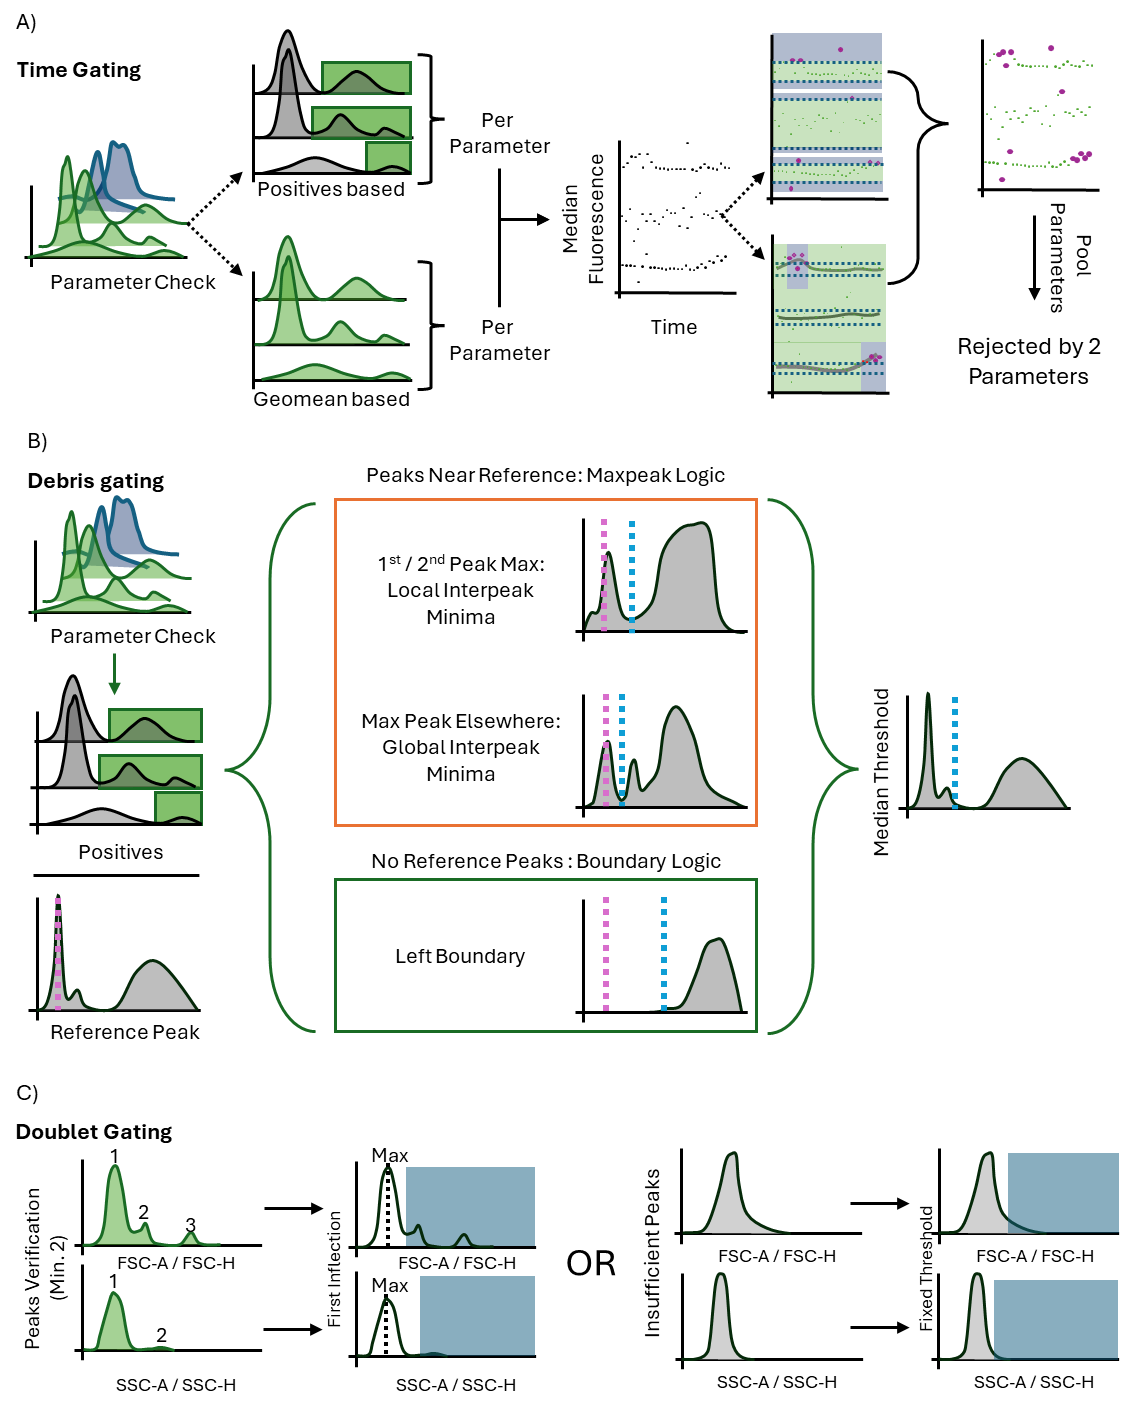
\includegraphics[width=\linewidth,height=0.82\textheight,keepaspectratio]{FlowMOP_submission_media/image1.png}
\begingroup
\renewcommand{\thefigure}{1}
\caption{Conceptual schematics depicting FlowMOP's time-gating (A), debris-gating (B), and doublet-gating (C) methods; plotted fluorescence intensity and signal-strength axes are schematic and use arbitrary units. A) FlowMOP selects valid parameters using positive-peak detection, generates time-binned fluorescence summaries, applies two smoothing resolutions, and performs robust outlier rejection across acquisition order. B) FlowMOP applies the same valid-parameter check, derives a candidate FSC-A threshold from each eligible parameter's positive events, and uses the median candidate as the final FSC-A gate. C) FlowMOP identifies doublets from inflection points in FSC-A/FSC-H and SSC-A/SSC-H ratio histograms, with a fixed-ratio fallback.}
\endgroup
\end{figure}

\subsection{Algorithmic design}\label{algorithmic-design}

An overview of FlowMOP's architecture is contained in Fig. 1, detailing
approaches for its preprocessing, time-gating, debris removal, and
doublet removal methods. This cleaned data can be applied to downstream
analysis.

FlowMOP accepts \texttt{.csv}, \texttt{.fcs}, and Parquet files. It
reduces event-level measurements into time-bin and channel summaries,
applies smoothing and robust outlier detection, and combines the
resulting flags through parameter voting.

\subsubsection{Precleaning}\label{precleaning}

FlowMOP first checks the input file for events at the limit of
detection, defined here as events at the maximum FSC-A value for that
sample. If the number of events at this maximum exceeds a threshold
(default 1\%), FlowMOP removes these maximum-valued events. Otherwise,
it retains all values. The 1\% cutoff is a pragmatic safeguard intended
to identify non-trivial accumulation at the acquisition maximum without
responding to isolated maximum-valued events.

\subsubsection{Time Gating}\label{time-gating}

To time gate, FlowMOP builds upon the assumptions posited in PeacoQC and
FlowCut regarding fluorescence fluctuations. That is, independent of
flow rate variations, sections of acquired sample with aberrant positive
fluorescence averages are the target portions to be removed. To achieve
this, FlowMOP checks each parameter, excluding parameters with a
unimodal distribution. `Unimodal distribution' is presently defined as
parameters with only one identifiable peak. Subsequently, for each
fluorescence parameter that satisfies this criterion, FlowMOP excludes
the first peak (selecting all subsequent peaks) and measures the average
fluorescence value for each time bin. FlowMOP then can operate either in
the `Positives' mode, or `Geomean' mode. In `Positives' mode, all events
before the first inflection point are discarded. All results shown
presently operate in `Positives' mode. In the `Geomean' mode, all events
are considered. Subsequently, on a per-parameter basis, the sample is
transformed into bins grouped by time (the default being bin having
minimum of 150 events, up to a maximum of 500 bins).

The median fluorescence of each bin's cells is returned. Two spline
smoothing values, one small and one larger (current default
\texttt{0.01,0.05}), are applied to the returned time-bin series before
median absolute deviation (MAD) filtering. The smoothing factor scales
the spline fit used for the binned fluorescence summary. Bins falling
outside the MAD threshold in either smoothing pass are flagged for
removal. Time-bins across all parameters are then combined, with time
bins rejected if they have been flagged in any parameter. For panels
with more than 10 parameters, FlowMOP requires two or more parameters to
flag a bin before rejection. This empirical safeguard reduces
false-positive removal caused by isolated noisy channels in
high-dimensional panels, although an aberration confined to one channel
may consequently be retained (Figure 1A).

FlowMOP summarizes each time bin using the median fluorescence of the
selected positive population. If Geomean mode is selected, FlowMOP
instead uses the geometric mean of all events in the bin. The two
smoothing resolutions target both shorter and more sustained deviations,
while parameter voting limits removal driven by isolated noisy channels
in higher-dimensional panels.

\subsubsection{Debris Gating}\label{debris-gating}

FlowMOP's debris module targets small, low-FSC debris. The final gate is
applied on FSC-A, but its threshold is informed by FSC-A distributions
across eligible fluorescence-positive populations rather than the
overall FSC-A histogram alone. SSC-A may improve recognition of larger
or internally complex debris, while pulse-width measurements may assist
with aggregates. Accordingly, FlowMOP does not currently incorporate
SSC-A or pulse-width measurements into its debris decision because
broadly applicable thresholds for these features are difficult to
establish across tissues, panels, instruments, and acquisition settings.
FlowMOP's debris exclusion conducts a similar unimodality check on each
fluorescence parameter, and the first peak is then excluded as the
Time-gating feature. Thereafter, FlowMOP detects the global FSC-A peak
as a reference point. For every parameter's positive events, FlowMOP
checks first for an FSC-A peak similar to the reference peak (default
30\% of the reference peak's value). If there is such a peak, it checks
if the second FSC-A peak is the global maximum FSC-A peak. If that
parameter's positive cell's second FSC-A is the global maxima, FlowMOP
returns the FSC-A threshold as the minima between those two FSC-A peaks.
If the second FSC-A is not the maximum, it returns the global interpeak
minimum between the reference peak and maximal peak. Conversely, if
there is no reference peak present in that parameter's positive
population, it selects the left-boundary of that parameter's first peak.
The median FSC-A threshold across all parameters is taken as the final
FSC-A gate to be applied to the sample (Figure 1B).

\subsubsection{Doublet Gating}\label{doublet-gating}

To doublet gate, FlowMOP dynamically excludes sample doublets. To do
this, FlowMOP creates a histogram of the FSC-A/FSC-H ratio. If there are
multiple peaks all with a ratio of 1 or more, then it chooses the
inflection point between those peaks, and excludes all events larger
than that value. If there are insufficient peaks, it simply returns all
events that have an FSC-A/FSC-H ratio smaller than a threshold (default
5). The process is repeated for the SSC-A/SSC-H variable. Consequently,
FlowMOP is able to distill the implicit ratiometric information that
current density based methodologies may overlook.
FlowMOP\textquotesingle s doublet module assumes that FSC-A/FSC-H and
SSC-A/SSC-H ratios remain informative and that acquisition voltages and
scatter parameters have been set appropriately. If relevant scatter
channels are saturated, edge-collapsed, or incorrectly configured at
acquisition, the lost pulse-shape information cannot be recovered by
FlowMOP or by other downstream preprocessing algorithms; such samples
require acquisition review, manual intervention, or alternative
pulse-shape features where available.

\subsection{Algorithmic Validation}\label{algorithmic-validation}

\subsubsection{Synthetic Sample
Benchmarking}\label{synthetic-sample-benchmarking}

The ability of FlowMOP to successfully detect time, debris, and
doublet-perturbed data was first tested against the respective task's
synthetic datasets, namely the synthetically combined staining time
samples, the high-debris + low debris samples, and the CTV / CFSE
doublet samples.

For time-gating samples, sensitivity and specificity were reported for
each benchmarked method using source labels as the reference. Target
source(s) were defined as the source(s) with the largest
filename-encoded mixture proportion; tied largest proportions were
treated as co-targets. Sensitivity was defined as retained target-source
events divided by all retained events. Specificity was defined as
removed non-target-source events divided by all removed events.

\begin{figure}[p]
\centering
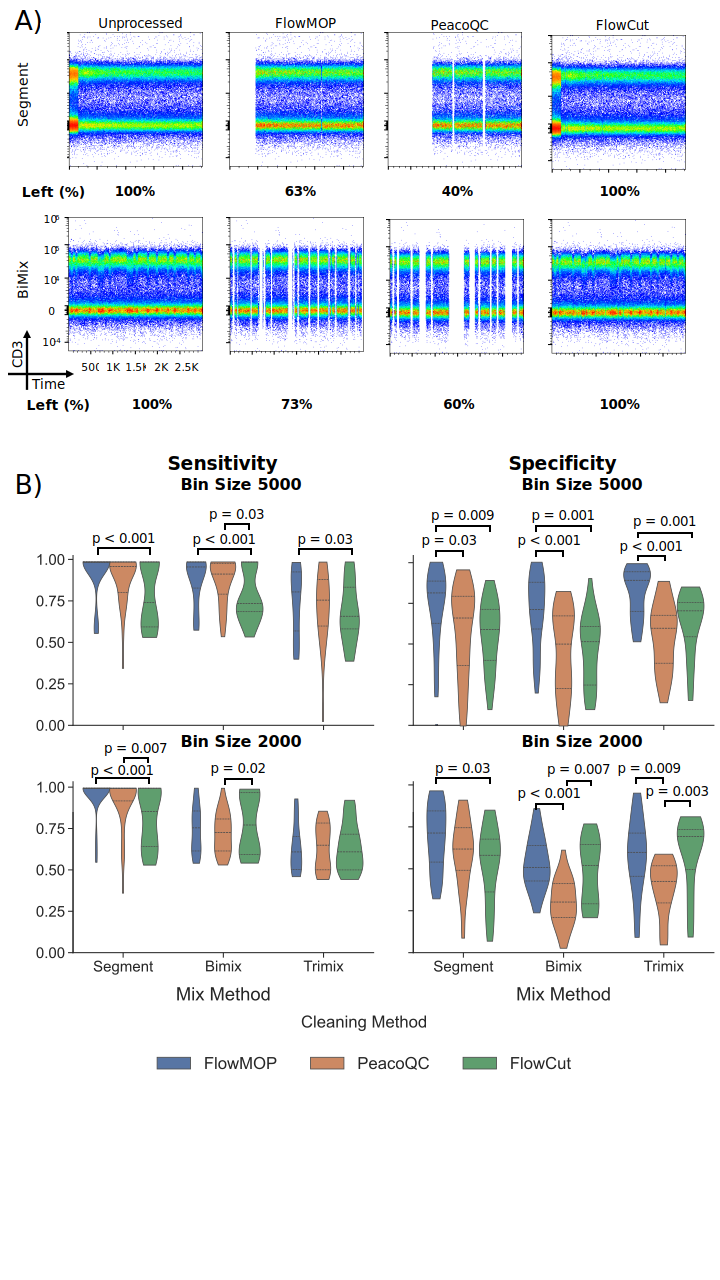
\includegraphics[width=\linewidth,height=0.82\textheight,keepaspectratio]{figs_data/figure_2.png}
\begingroup
\renewcommand{\thefigure}{2}
\caption{A) Representative flow cytometry plots showing CD3 fluorescence against time. The original synthetically generated sample is shown in column 1, with the resulting output following FlowMOP, PeacoQC, and FlowCut processing shown in the subsequent columns. The first row depicts a representative `segmentation'-based synthetic file. The second row shows a representative two-sample mixture with a 5000-event bin size. Frequency percentages shown are the percentage of cells left post-cleaning relative to the original synthetic sample (rounded to the nearest percentage point). B) Violin plots showing sensitivity and specificity, grouped by sample type (Segment, Bimix, and Trimix) and cleaning method (FlowMOP, PeacoQC, and FlowCut). Internal dashed lines indicate quartiles. The first and second rows represent mixing-bin sizes of 5000 events (n = 90: Segment, 33; Bimix, 33; Trimix, 24) and 2000 events (n = 83: Segment, 32; Bimix, 28; Trimix, 23), respectively. Brackets show significant Bonferroni-adjusted paired t-tests.}
\endgroup
\end{figure}

\subsubsection{Synthetic Time Gating
Benchmark}\label{synthetic-time-gating-benchmark}

Several computational approaches address time-dependent quality control,
including flowAI {[}10{]}, PeacoQC {[}5{]}, flowClean {[}6{]}, and
FlowCut {[}9{]}. FlowMOP combines a time-gating component with debris
and doublet modules in one Python workflow. Here, its time-gating
performance is evaluated against PeacoQC and FlowCut.

The Segment, Bimix, and Trimix samples were designed as complementary
time-artifact stress tests with event-level source information for
objective scoring (Fig. 2A). Sensitivity was defined as the proportion
of retained events derived from the target source or sources, and
specificity as the proportion of removed events derived from the
non-target source or sources. Direct comparison with manual gating was
not attempted because the short, interspersed intervals in the Bimix and
Trimix samples are impractical to remove reproducibly by eye.

At the 5000-event bin size, FlowMOP had higher sensitivity than FlowCut
in Segment (p \textless{} 0.001), Bimix (p \textless{} 0.001), and
Trimix (p = 0.03) (Fig. 2B). PeacoQC also had higher sensitivity than
FlowCut in Bimix (p = 0.03). FlowMOP had higher specificity than both
PeacoQC and FlowCut in Segment (p = 0.03 and p = 0.009), Bimix (p
\textless{} 0.001 and p = 0.001), and Trimix (p \textless{} 0.001 and p
= 0.001), respectively.

At the 2000-event bin size, FlowMOP and PeacoQC had higher sensitivity
than FlowCut in Segment (p \textless{} 0.001 and p = 0.007,
respectively), while FlowMOP had higher specificity than FlowCut (p =
0.03). In Bimix, PeacoQC had lower sensitivity than FlowCut (p = 0.02)
and lower specificity than both FlowMOP (p \textless{} 0.001) and
FlowCut (p = 0.007). In Trimix, sensitivity did not differ significantly
among methods, while PeacoQC had lower specificity than FlowMOP (p =
0.009) and FlowCut (p = 0.003). All comparisons were paired t-tests with
Bonferroni correction, using each algorithm\textquotesingle s fixed
recommended or default settings.

To test the effect of flow-rate disturbances aligned with or independent
of source-linked fluorescence changes, we altered only the Time channel
while leaving fluorescence, scatter, source labels, and event order
unchanged (Fig. S4). FlowMOP and PeacoQC were unchanged under both
source-linked and random Time warping. In contrast,
FlowCut\textquotesingle s sensitivity and specificity shifted after
Time-only perturbation. Across all inputs, random Time warping reduced
FlowCut\textquotesingle s specificity by 11.45 percentage points
relative to matched raw inputs. In Segment inputs, source-linked Time
warping reduced FlowCut\textquotesingle s sensitivity by 7.84 percentage
points and specificity by 15.25 percentage points. These results support
the interpretation that FlowCut responds to local acquisition-density
structure even when fluorescence values are unchanged, whereas FlowMOP
and PeacoQC are unaffected by rate-only variation in these inputs.

Dual-resolution smoothing changed the balance between sensitivity and
specificity (Table S4). The no-smoothing control had the highest
equal-weight balanced mean (0.7551), but its sensitivity was 1.92
percentage points lower than that of \texttt{0.01,0.05}. Among smoothed
settings, \texttt{0.01,0.05} had the highest balanced mean (0.7511),
with specificity 2.70 percentage points lower than the no-smoothing
control. We therefore selected \texttt{0.01,0.05} as the default and
regenerated Figure 2 using this setting.

Representative plots for the 2000 bin Bimix method, and the 2000, and
5000 bin Trimix methods can be found in Supp. 1.

\subsubsection{Computational
scalability}\label{computational-scalability}

Clone-based runtime and memory benchmarking showed that FlowMOP scaled
favorably at larger event counts (Table 1). Values are mean ± SD across
three measured repeats after one warm-up run. FlowMOP was fastest from
100,000 events onward and had the lowest peak RAM at all sizes except
100,000 events. At 1,000,000 events, FlowMOP completed in 10.69 ± 0.16
s, compared with 24.21 ± 0.23 s for PeacoQC and 30.34 ± 0.48 s for
FlowCut, while using 658.0 ± 0.3 MB peak RAM compared with 1483.4 ± 86.8
MB and 1115.1 ± 0.3 MB. At 2,000,000 events, FlowMOP completed in 17.42
± 0.88 s, compared with 43.18 ± 4.23 s and 60.61 ± 2.37 s, while using
839.5 ± 0.4 MB peak RAM compared with 2614.8 ± 0.1 MB and 1849.8 ± 0.3
MB.

\clearpage
\begingroup
\scriptsize
\setlength{\tabcolsep}{2pt}
\renewcommand{\arraystretch}{1.10}

\captionsetup{type=table}
\begingroup
\renewcommand{\thetable}{1}
\captionof{table}{\textbf{Clone-based time-gating runtime and memory benchmark}}
\endgroup

Mean runtime and peak RAM across three measured repeats are shown as
mean ± SD. The best-performing runtime and RAM value for each event
count is shown in bold.

{\def\LTcaptype{none} % do not increment counter
\begin{longtable}[]{@{}
  >{\raggedleft\arraybackslash}p{(\linewidth - 12\tabcolsep) * \real{0.1371}}
  >{\raggedleft\arraybackslash}p{(\linewidth - 12\tabcolsep) * \real{0.1371}}
  >{\raggedleft\arraybackslash}p{(\linewidth - 12\tabcolsep) * \real{0.1371}}
  >{\raggedleft\arraybackslash}p{(\linewidth - 12\tabcolsep) * \real{0.1371}}
  >{\raggedleft\arraybackslash}p{(\linewidth - 12\tabcolsep) * \real{0.1371}}
  >{\raggedleft\arraybackslash}p{(\linewidth - 12\tabcolsep) * \real{0.1371}}
  >{\raggedleft\arraybackslash}p{(\linewidth - 12\tabcolsep) * \real{0.1371}}@{}}
\toprule\noalign{}
\begin{minipage}[b]{\linewidth}\raggedleft
Events
\end{minipage} & \begin{minipage}[b]{\linewidth}\raggedleft
FlowMOP time (s)
\end{minipage} & \begin{minipage}[b]{\linewidth}\raggedleft
PeacoQC time (s)
\end{minipage} & \begin{minipage}[b]{\linewidth}\raggedleft
FlowCut time (s)
\end{minipage} & \begin{minipage}[b]{\linewidth}\raggedleft
FlowMOP RAM (MB)
\end{minipage} & \begin{minipage}[b]{\linewidth}\raggedleft
PeacoQC RAM (MB)
\end{minipage} & \begin{minipage}[b]{\linewidth}\raggedleft
FlowCut RAM (MB)
\end{minipage} \\
\midrule\noalign{}
\endhead
\bottomrule\noalign{}
\endlastfoot
10,000 & 2.67 ± 0.50 & 4.40 ± 0.57 & \textbf{1.72 ± 0.02} &
\textbf{237.9 ± 0.2} & 446.6 ± 0.2 & 261.8 ± 0.3 \\
100,000 & \textbf{4.34 ± 0.11} & 13.74 ± 1.34 & 4.78 ± 0.33 & 351.6 ±
0.1 & 606.6 ± 26.1 & \textbf{326.4 ± 0.1} \\
300,000 & \textbf{8.42 ± 0.85} & 15.08 ± 0.84 & 10.91 ± 0.49 &
\textbf{462.3 ± 0.4} & 948.5 ± 5.9 & 505.4 ± 0.4 \\
1,000,000 & \textbf{10.69 ± 0.16} & 24.21 ± 0.23 & 30.34 ± 0.48 &
\textbf{658.0 ± 0.3} & 1483.4 ± 86.8 & 1115.1 ± 0.3 \\
2,000,000 & \textbf{17.42 ± 0.88} & 43.18 ± 4.23 & 60.61 ± 2.37 &
\textbf{839.5 ± 0.4} & 2614.8 ± 0.1 & 1849.8 ± 0.3 \\
\end{longtable}
}

\endgroup

\subsubsection{Synthetic Debris Gating
Benchmark}\label{synthetic-debris-gating-benchmark}

\begin{figure}[p]
\centering
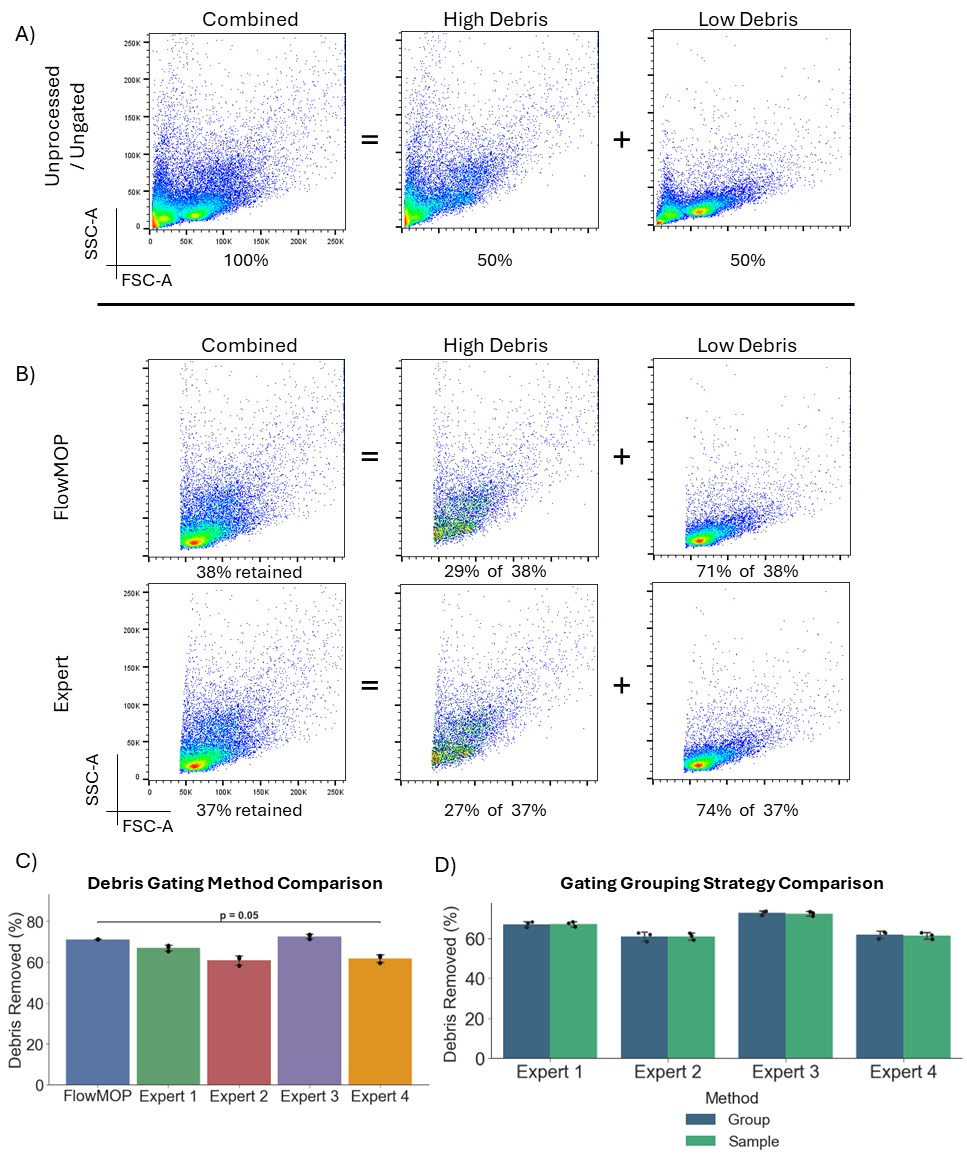
\includegraphics[width=\linewidth,height=0.82\textheight,keepaspectratio]{FlowMOP_submission_media/image3.png}
\begingroup
\renewcommand{\thefigure}{3}
\caption{A) Representative flow cytometry plots showing FSC-A/SSC-A debris plots. The first plot represents a representative combined high + low debris sample, the second and third represent the high debris portion and the low debris portion of that sample respectively. The percentages below denote the proportion of the combined sample represented by the annotated plot. B) FSC-A/SSC-A flow plots of the Fig. 3A's representative sample post-processing. Again, the first column shows the combined high + low debris sample, the second and third show the high debris and low debris samples separately respectively. The percentages in the first column denote the proportion of the sample remaining relative to the original combined sample. Percentages in the high debris and low debris columns denote the post-filtering proportion that each comprises (rounded to the nearest percentage). C) Bar plot representing mean proportion percentage ± SD of low debris sample remaining post-processing for FlowMOP and four human experts. FlowMOP has significantly higher low debris sample proportion than Expert 4 (Bonferroni adjusted paired t-test, p = 0.04). D) Bar plots showing mean low debris sample proportion percentage ± SD following human expert gating using either a group or per-sample based strategy (Blue bars denote group-wise results, green sample-wise). No difference was found between the two methods (un-adjusted paired t-test, p \textgreater{} 0.05).}
\endgroup
\end{figure}

FlowMOP's debris gating performance was tested by its ability to deplete
the high-debris component in the combined high- and low-debris samples
(Fig. 3A). FlowMOP reduced the high-debris source proportion from 50 ±
1.10\% to 28.8 ± 0.1\% (paired t-test, p \textless{} 0.001) (Fig. 3B).
The final gate is applied on FSC-A, but its threshold is derived from
candidate FSC-A distributions across eligible fluorescence-positive
populations rather than from the overall FSC-A histogram alone. FlowMOP
did not differ significantly from any human evaluator except Expert 4,
for whom FlowMOP removed more labelled high-debris events
(Bonferroni-adjusted paired t-test, p = 0.04) (Fig. 3C).

FlowMOP by default conducts debris removal on a per-sample basis. For
comparison with the standard per-group gating methodology, human experts
were also requested to apply per-sample and per-group gating strategies
for comparison. No difference was found between per-sample and
group-based gating for any expert (Fig. 3D, unadjusted paired t-Test p
\textgreater{} 0.05).

\subsubsection{Synthetic Doublet Gating
Benchmark}\label{synthetic-doublet-gating-benchmark}

FlowMOP's doublet removal performance was also examined through
synthetic technical controls (Fig. 4A). Events positive for both CFSE
and CTV provide an observable class of heterologous labelled doublets,
subject to rare dye-transfer events; same-label CTV-CTV and CFSE-CFSE
doublets are not identifiable from these labels alone. FlowMOP was then
run on these samples, and the proportion of remaining CFSE/CTV
double-positive cells was compared with the proportions remaining after
human-expert gating (Fig. 4A).

\begin{figure}[p]
\centering
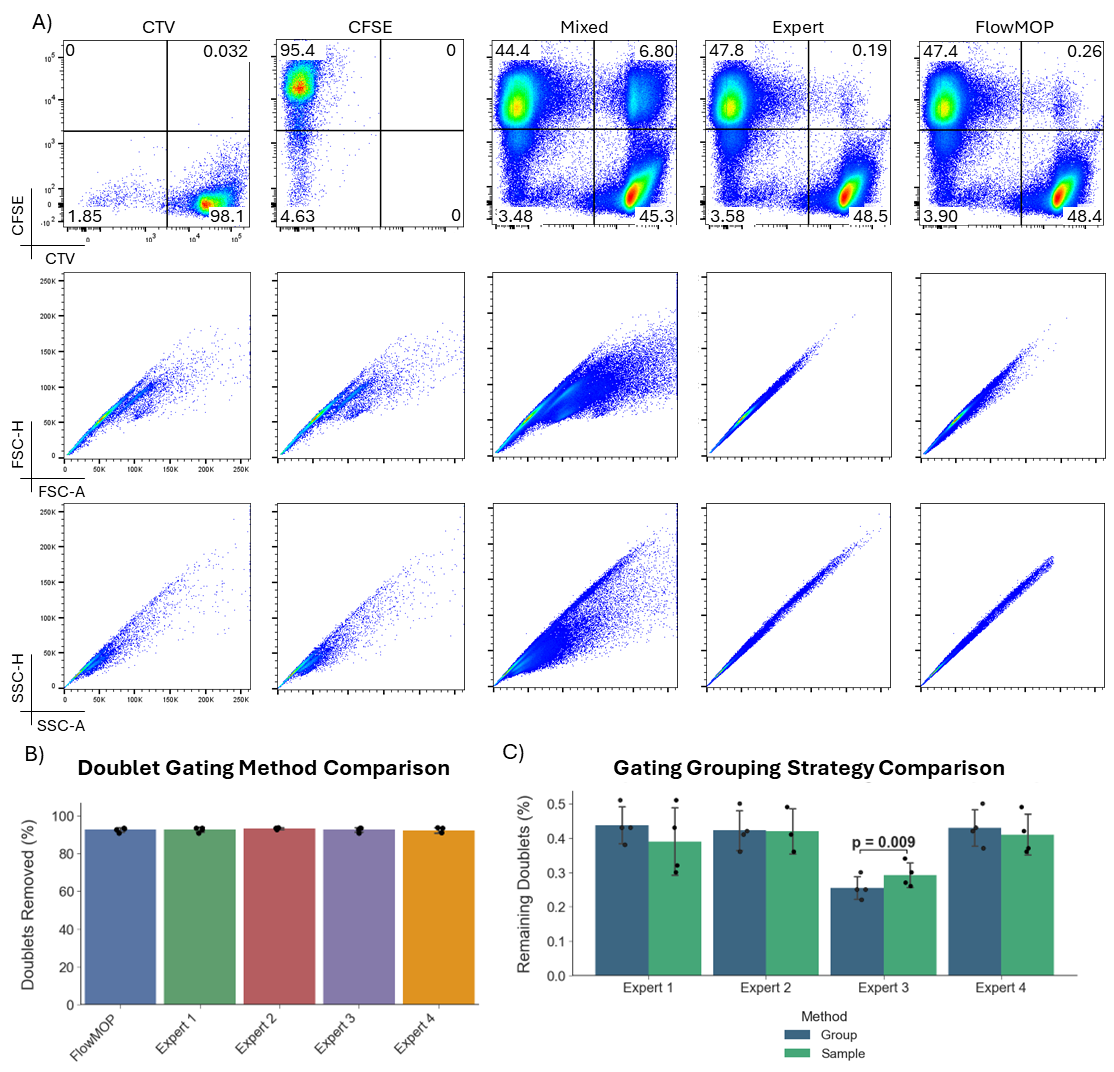
\includegraphics[width=\linewidth,height=0.82\textheight,keepaspectratio]{FlowMOP_submission_media/image4.png}
\begingroup
\renewcommand{\thefigure}{4}
\caption{A) Representative flow cytometry plots of synthetic doublet samples and gating. The first row shows all samples by CTV against CFSE, the second FSC-A/FSC-H, and the last by SSC-H/SSC-A. The columns show representative CTV-only stained, CFSE-only stained, mixed CTV-CFSE, human expert doublet-removed, and FlowMOP doublet removed samples. B) Bar graph showing the mean percentage ± SD of CTV-CFSE double positive events removed (relative to the original sample) following FlowMOP or human expert processing. C) Bar graphs showing mean frequency ± SD of remaining CTV-CFSE double positive events following human expert processing, comparing group and per-sample based gating strategies (Blue bars denote group-wise results, green sample-wise). Only Expert 3 had significantly different results (un-adjusted paired t-test, p = 0.001, all others p \textgreater{} 0.05).}
\endgroup
\end{figure}

FlowMOP significantly decreased the frequency of CTV-CFSE
double-positive events from 7.84 ± 1.21\% to 0.27 ± 0.11\% (paired
t-test; p = 0.001). No statistically significant difference was detected
between FlowMOP and any expert for this endpoint (Fig. 4B, paired
t-test; unadjusted p \textgreater{} 0.05). To assess whether sample-wise
gating systematically affected the comparison, human experts also
performed sample-wise and groupwise doublet gating. No statistical
difference was detected between these approaches except for Expert 3
(Fig. 4C, paired t-test; unadjusted p values). Expert 3 consistently
removed fewer doublets with the sample-wise method than with the group
method (Fig. 4C, paired t-test; p = 0.009).

\subsection{Biological validation}\label{biological-validation}

Following the objective synthetic benchmarks, FlowMOP will be evaluated
using prespecified biological population endpoints in biological
flow-cytometry datasets.

\textbf{{[}PLACEHOLDER: Figure 5 biological-validation cohort,
endpoints, results, and statistical comparisons.{]}}

\textbf{{[}PLACEHOLDER: Figure 5. Biological validation of FlowMOP
cleaning.{]}}

\subsection{Tumour-liver acquisition instability and downstream
biological
concordance}\label{tumour-liver-acquisition-instability-and-downstream-biological-concordance}

\textbf{{[}PLACEHOLDER: Final Figure 6 analysis and corresponding text
from Felix\textquotesingle s tumour-validation dataset.{]}}

In the three tumour-liver files, FlowMOP identified the principal
acquisition intervals with strong multichannel fluorescence instability,
including the major disturbances identified by manual gating, FlowCut,
or PeacoQC. FlowMOP also identified additional intervals with shifts in
positive-population fluorescence, whereas residual intervals detected
only by comparator methods generally showed weaker fluorescence
divergence. The substantial overlap between retained and removed events
at the individual-event level indicates that the time gate detected
acquisition-dependent shifts in population summaries rather than a
discrete aberrant cell phenotype.

These findings also demonstrate that acquisition instability was not
confined to conspicuous beginning- or end-of-run departures: the
biological files contained mid-acquisition intervals with coordinated
fluorescence shifts, including subtle intervals that would be difficult
to define reproducibly by visual gating alone.

Across the three tumour and three non-tumour liver samples, the combined
FlowMOP time, debris, and doublet masks retained 61.1\% ± 10.0\% of
events, compared with 51.3\% ± 17.8\% after reconstructed manual gating
(Tables S3A-B). FlowMOP had greater permissiveness-adjusted Zombie-high
removal selectivity than manual gating in four of six samples. The
median paired FlowMOP/manual selectivity fold-change was 1.68 (range
0.82-2.70), but the difference was not statistically significant (exact
two-sided Wilcoxon signed-rank test on log ratios, p = 0.156). Thus,
this analysis detected neither systematic superiority nor inferiority
relative to manual gating; it was not designed to establish statistical
equivalence.

Decomposition of the FlowMOP workflow showed distinct contributions from
its three masks. The time mask was approximately composition-neutral
(median Zombie-high/Zombie-low removal ratio 1.04), and debris removal
was heterogeneous across samples. The doublet mask preferentially
excluded Zombie-high events in all six samples (median ratio 7.38;
secondary exact two-sided paired test, p = 0.031), making it the
principal source of Zombie-high enrichment in the combined output. The
doublet inflection procedure used its prespecified MAD fallback in these
files, so this association provides biological concordance for the
resulting mask but does not establish that every removed event was an
invalid doublet.

\textbf{{[}PLACEHOLDER: Figure 6. FlowMOP validation in tumour-derived
biological samples.{]}}

\FloatBarrier

\section{Discussion}\label{discussion}

FlowMOP was evaluated for time, debris, and doublet gating using
synthetic technical controls and biological datasets.

\subsection{Synthetic Benchmarking}\label{synthetic-benchmarking}

\subsubsection{Synthetic Sample Time
Gating}\label{synthetic-sample-time-gating}

In the synthetic time-gating analysis, the Segment time gate is perhaps
the most common and consequential time-artifact, as a non-negligible
sample portion is often required to be removed in real samples. This
type of synthetic data expects gating most similar to current manual
gating, where blocks of events are removed. The objective of these
samples is to simulate where there is a long blockage or sudden shift in
the acquired sample. Here, FlowMOP had higher sensitivity than FlowCut
at both tested bin sizes. It also had higher specificity than both
competitors at 5000 events and than FlowCut at 2000 events. The
Time-only mechanism benchmark suggests that the FlowMOP versus FlowCut
difference is not explained solely by implementation. When local
acquisition-rate structure was altered either in alignment with
source-linked fluorescence changes or independently of them, FlowMOP
remained unchanged, whereas FlowCut\textquotesingle s removal behavior
shifted, especially in Segment inputs (Fig. S4). This supports the
interpretation that FlowCut can be affected by acquisition-density
changes even when fluorescence values are unchanged, while FlowMOP is
more anchored to fluorescence-population summaries across acquisition
order.

Transient acquisition disturbances are not confined to the beginning or
end of a run: flow-rate surges interspersed throughout acquisition and
associated signal-intensity variation have been documented {[}10{]}.
PeacoQC notes that temporary acquisition problems can be difficult to
detect manually {[}5{]}, and FlowCut describes manual identification and
removal of transient acquisition problems as time-consuming and
subjective {[}9{]}. We use ``microblockage'' operationally for a short,
self-resolving instance of this broader phenomenon that produces a
localized fluorescence shift, without asserting that a physical
obstruction was directly observed. The Bimix and Trimix samples were
designed to represent this under-addressed case. Although these
synthetic samples can appear acceptable on visual inspection, the source
labels show that the short altered intervals contain events from an
intentionally perturbed fluorescence source and therefore should be
excluded under the benchmark definition. Visual subtlety is thus a
central feature of the benchmark: it demonstrates why apparent normality
by eye is not sufficient ground truth. The tumour-liver validation
further supports the experimental relevance of this design by
demonstrating mid-acquisition intervals with coordinated multichannel
fluorescence shifts.

The size of the simulated microblockage was determined by the mixing-bin
size, with the 2000-event samples representing shorter and more
difficult disturbances than the 5000-event samples. FlowMOP provided the
strongest overall performance profile across these conditions. At 5000
events, it had higher sensitivity than FlowCut and higher specificity
than both competitors across Segment, Bimix, and Trimix. At 2000 events,
FlowMOP had higher sensitivity and specificity than FlowCut in Segment
and retained higher specificity than PeacoQC in Bimix and Trimix without
a significant sensitivity disadvantage. Thus, FlowMOP\textquotesingle s
principal advantage was its consistent combination of high sensitivity
with stronger specificity across sustained and short, interspersed time
artifacts.

PeacoQC\textquotesingle s documentation identifies acquisition-bin size
as a trade-off between the accuracy of within-bin density estimation,
the number of bins available for evaluating signal stability, and the
number of events affected when a bin is removed {[}5{]}. The Bimix and
Trimix benchmarks contain short, interspersed source-defined intervals.
FlowMOP\textquotesingle s stronger performance is therefore consistent
with its temporal summarisation being better matched to these brief
intervals.

The computational benchmark demonstrates that FlowMOP provides speed
gains with lower peak RAM usage at larger event counts. This is most
evident from 300,000 events onward, where FlowMOP had both the fastest
mean runtime and lowest peak memory use. At 2,000,000 events, FlowMOP
was approximately 2.5-fold faster than PeacoQC and 3.5-fold faster than
FlowCut, while using approximately 32\% of PeacoQC's peak RAM and 45\%
of FlowCut's peak RAM.

These measurements were obtained using local non-distributed execution
and therefore demonstrate the performance of the tested implementations,
not a distributed-computing speedup.

Among the three evaluated decision structures, only FlowMOP exposes an
inherently channel-parallel within-sample computation. After shared
acquisition bins are defined, each eligible fluorescence channel
independently establishes its reference, produces a fixed-shape time-bin
summary, and applies smoothing and MAD filtering; cross-channel
coordination occurs only in the final parameter vote. PeacoQC instead
performs data-dependent peak identification and reconciliation across
bin-channel combinations, while FlowCut applies adjacent-segment,
contiguous-region, file-wide, and conditional rerun decisions {[}5,9{]}.
Their suboperations and separate files can be parallelised, but their
complete within-sample decision pipelines cannot be expressed as the
same independent channel-wise reduction without changing their decision
rules. Porting either implementation to another language or scheduling
framework would therefore not remove these structural dependencies. This
structural distinction, together with FlowMOP's earlier data reduction,
fewer full-data passes, and smaller intermediate state, is consistent
with its lower runtime and memory use in our benchmarks, although the
benchmark does not independently establish causation.

It is of note that there is a large variation in algorithmic performance
across the dataset. One source of this variation is that the 0.5 and 1.0
relative cell concentrations oftentimes exhibited marginal differences
in fluorescence intensity (Supp. Fig. 3), especially relative to the 0.5
/ 3.0 cell concentrations comparison. Consequently, the 0.5/1.0
discrimination tasks can be considered especially difficult benchmarks
to overcome. However, this difficulty was intentionally placed, to
ensure the present benchmarking dataset could also show progressive
improvement of future time-gating algorithms.

Human gating was not included for the Bimix or Trimix synthetic datasets
because the short mixed bins do not provide a practical manual
ground-truth target. The retained source labels instead provide an
event-level reference for comparing algorithmic performance. A dataset
benchmark was therefore necessary to evaluate whether automated methods
can detect these subtle but labelled artifacts reproducibly.

\subsubsection{Synthetic Sample Debris and Doublet
Gating}\label{synthetic-sample-debris-and-doublet-gating}

In the synthetic debris and doublet gating trials, FlowMOP removed the
labelled technical artifact populations effectively (Fig. 3B, 4B). In
the debris task, FlowMOP enriched the low-debris component by 9.67\%,
which represented approximately 19\% more debris removed considering the
original 50:50 debris / real sample mixture. FlowMOP's debris
performance can also be interpreted in relation to the two debris
populations (Fig. 3A) present: one at \textless10,000 FSC-A units, and
the second at \textasciitilde20,000 FSC-A units. Human experts were
instructed that this second debris population was debris, and to gate
accordingly. FlowMOP was able to independently detect this second debris
population and exclude it without external information.

Similarly, in the doublet removal, the synthetic samples, owing to the
rather unique preparation, yielded triplets. FlowMOP was able to handle
this unexpected population and successfully removed it.

The synthetic debris benchmark measures depletion of the source-labelled
high-debris component from matched mixtures of high- and low-debris
samples. Because both sources contain some debris, these labels
represent relative debris enrichment rather than per-event debris
classification. FlowMOP targets the small, low-FSC debris phenotype
observed in these controls and successfully removed the two low-FSC
debris populations shown in Figure 3A. SSC-A may improve recognition of
larger or internally complex debris, while pulse-width measurements may
assist with aggregates. Accordingly, FlowMOP does not currently
incorporate these features because broadly applicable decision rules are
difficult to establish across tissues, panels, instruments, and
acquisition settings. Future extensions can evaluate configurable or
sample-specific multivariate approaches in tumour digests with greater
necrosis, aggregation, and scatter heterogeneity.

\subsection{Biological validation}\label{biological-validation-1}

\textbf{{[}PLACEHOLDER: Interpretation of the Figure 5
biological-validation endpoint and its implications for preservation of
biologically meaningful populations following cleaning.{]}}

\textbf{{[}PLACEHOLDER: Integrate Felix\textquotesingle s final Figure 6
tumour-validation findings here.{]}}

The tumour-liver analysis provides an initial downstream
biological-concordance assessment. FlowMOP retained more events on
average, while its permissiveness-adjusted Zombie-high selectivity was
statistically indistinguishable from the matched manual strategy in this
six-sample analysis. This result is compatible with similar performance
but does not demonstrate parity, because the analysis was not powered or
prespecified as an equivalence or non-inferiority test. The constituent
analysis further indicates that the complete workflow should not be
treated as a single biological filter: time gating detected
acquisition-level fluorescence instability without consistent Zombie
selectivity, debris effects were sample-dependent, and the doublet mask
generated most of the observed Zombie-high enrichment.

An earlier expert preference exercise across nine human and mouse
datasets is reported in Supplementary Figures S5-S7. The exercise used
an earlier FlowMOP configuration and involved one relevant expert per
tissue type. These rankings are therefore interpreted as exploratory
relative preferences rather than absolute quality scores or evidence of
the performance of the current implementation.

\subsection{Other remarks}\label{other-remarks}

Automated Live/Dead classification of events was considered, however not
implemented in the algorithm. There exist many varied protocols and
methods for discriminating live/dead samples, along with great diversity
in the determination of what constitutes a `dead' event. Consequently,
the difficulty of creating a universal live/dead discriminator is
non-trivial. Finally, there may be potential significant biological
insight in the `dead' cells of a sample, whereby important information
concerning a sample may be found in the dead events or their proportion.

The biological cost of preprocessing errors is difficult to measure
directly, and neither under-cleaning nor over-cleaning is preferable.
Under-cleaning may allow acquisition-time artifacts with abnormal
staining patterns to confound downstream results, including by creating,
inflating, or obscuring apparent rare populations. Conversely,
over-cleaning could remove rare or transient biological populations.
Because FlowMOP\textquotesingle s time-gating module operates on
acquisition-time structure rather than population identity, rare
populations are not expected to be systematically biased unless they are
temporally confounded with an acquisition artifact.

The primary comparison used recommended or automatically selected
settings, including fixed FlowMOP parameters, to reflect typical
unsupervised use.

CTV-CFSE double-positive events provide an observable ground-truth
doublet class, but same-label CTV-CTV and CFSE-CFSE doublets are not
directly detectable in this validation design. Instruments providing
multiple scatter measurements, including 405-nm, 488-nm, and polar
488-nm FSC/SSC configurations, were not evaluated here. Future versions
could assess multiple scatter-channel pairs and select or combine the
pair with the clearest debris/doublet separation.

\FloatBarrier

\section{Conclusion}\label{conclusion}

FlowMOP provides time-gating, conservative low-FSC debris removal, and
scatter-ratio doublet removal in a single Python implementation. This
facilitates integration with Python-based workflows and provides fast,
memory-conscious preprocessing for large cytometry files.

Within the tested synthetic scenarios, event-level source labels enabled
objective evaluation of the targeted artifact classes. FlowMOP had
higher sensitivity than FlowCut for Segment anomalies at both bin sizes
and higher specificity than both competitors across the 5000-event
Segment, Bimix, and Trimix benchmarks. For debris and doublet removal,
FlowMOP removed the labelled technical artifact populations effectively
in the synthetic ground-truth datasets, including unexpected triplet
events.

An exploratory expert comparison using an earlier FlowMOP configuration
generally favoured manual gates and is reported in the Supplementary
Information. \textbf{{[}PLACEHOLDER: Figure 5 biological-validation
conclusion.{]}} \textbf{{[}PLACEHOLDER: Figure 6 tumour-validation
conclusion.{]}} The open-source Python implementation supports
reproducible preprocessing across cytometry datasets of increasing
scale.

\FloatBarrier

\section{Data and Code Availability}\label{data-and-code-availability}

FlowMOP can be accessed via
\url{https://github.com/1ordinateur/FlowMOP}. The code associated with
the creation of this paper can be accessed at
\url{https://github.com/1ordinateur/FlowMOP_paper}. The FCS Files used
for this paper can be accessed at
\url{http://doi.org/10.5281/zenodo.17896445}.

\FloatBarrier

\clearpage

\section{Supplementary data}\label{supplementary-data}

\begin{figure}[p]
\centering
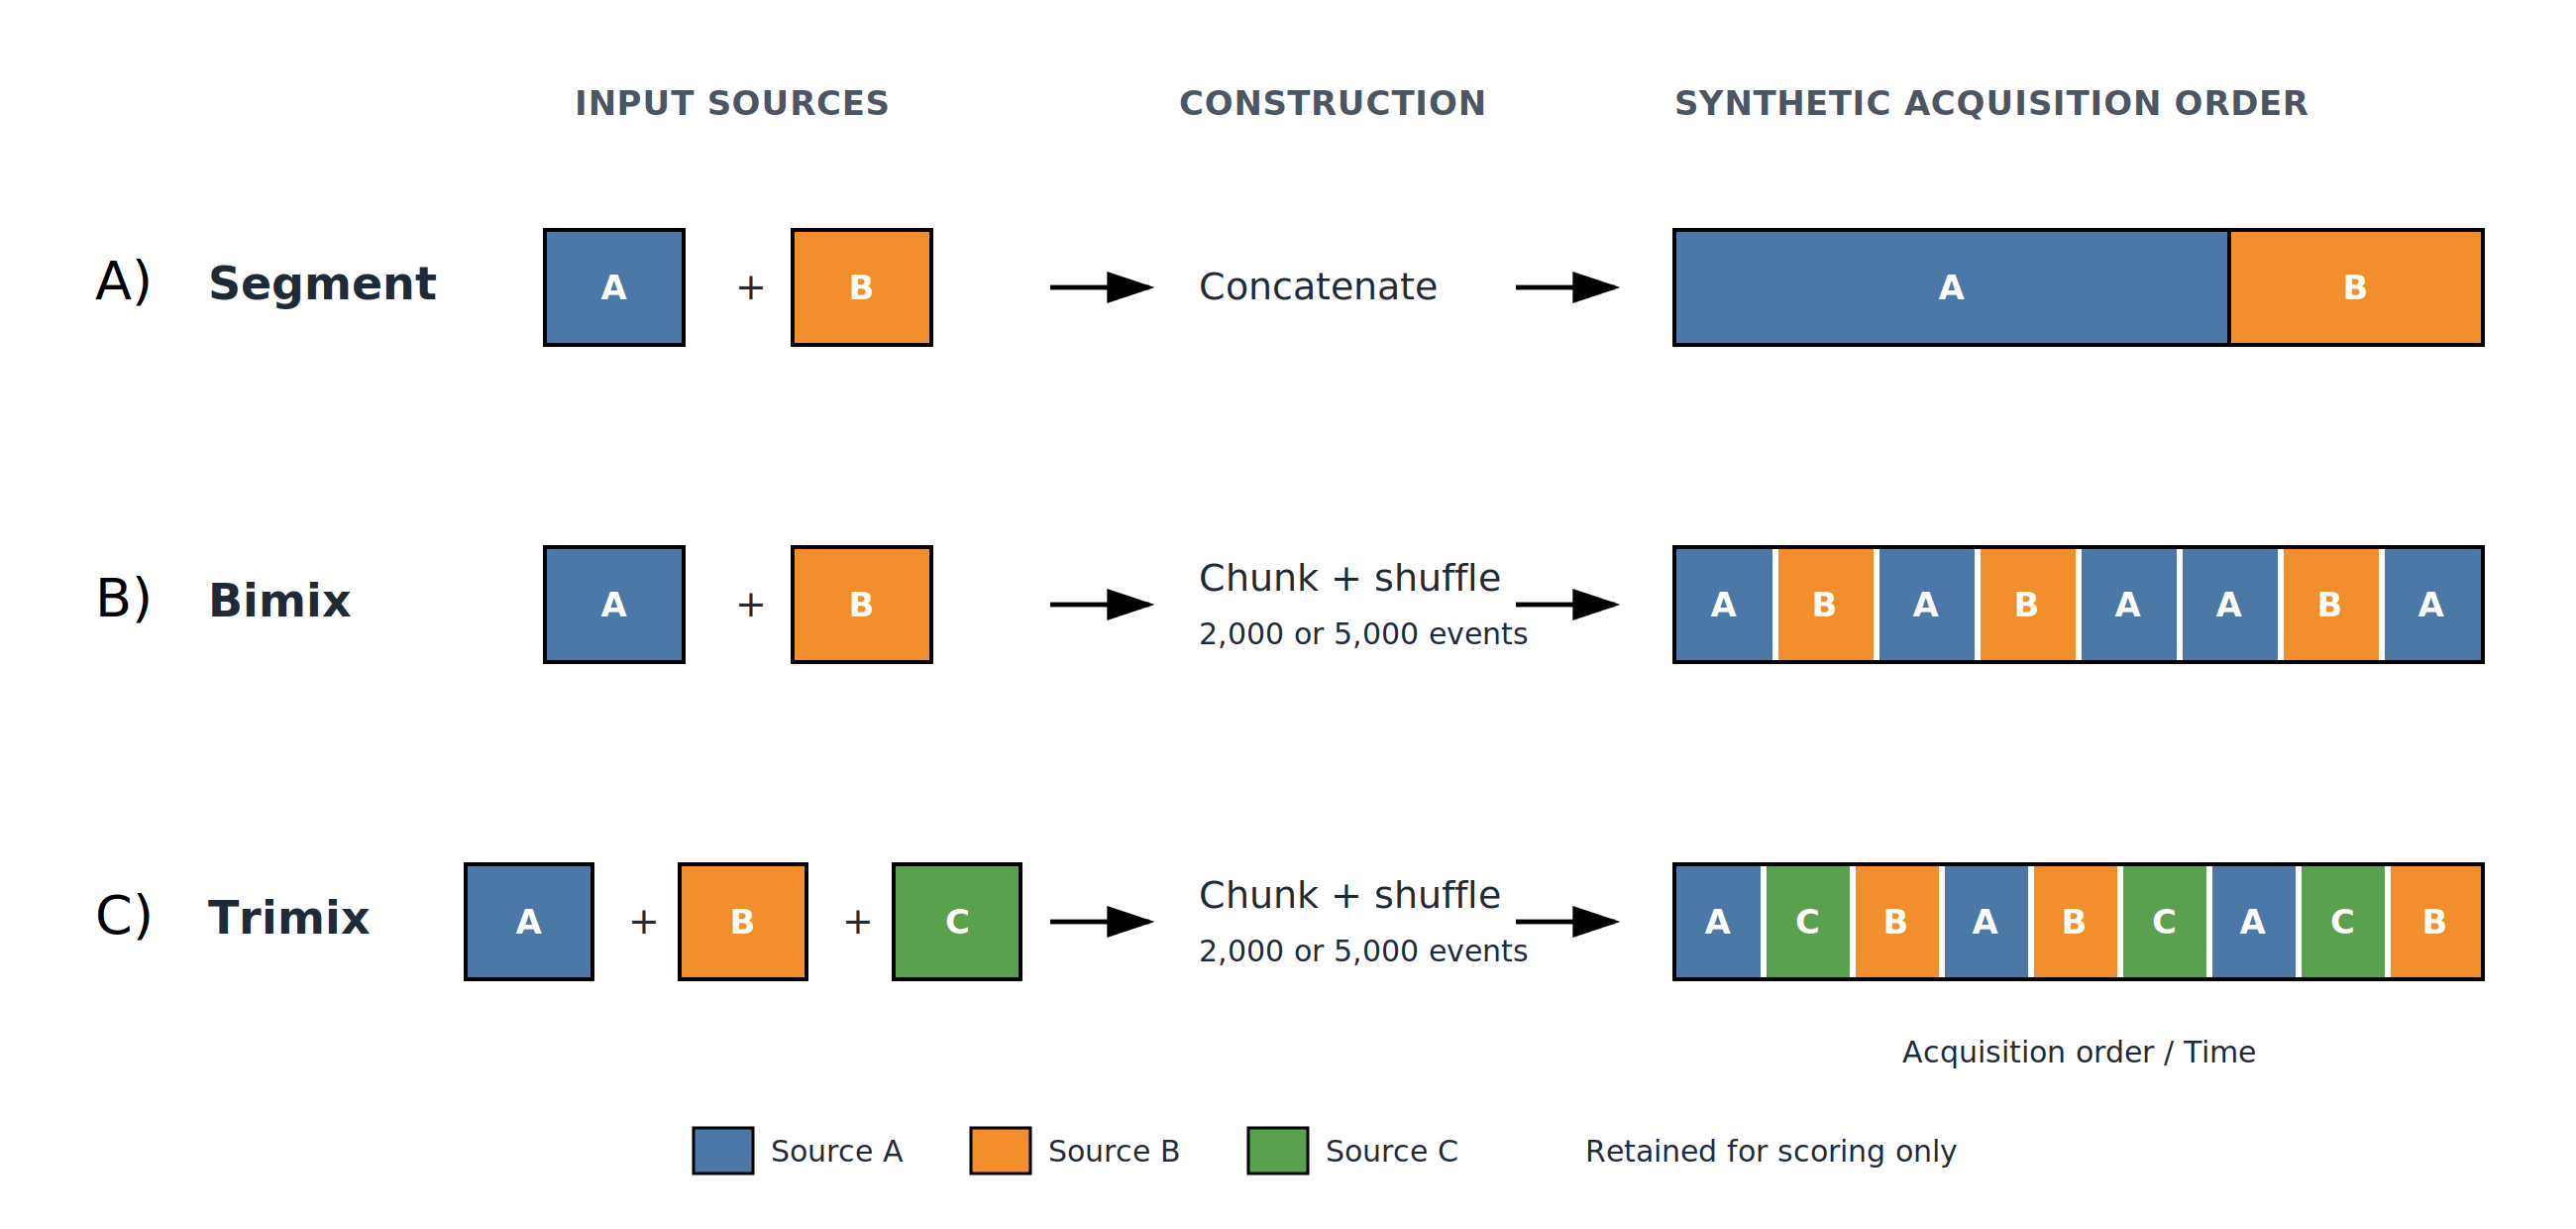
\includegraphics[width=\linewidth,height=0.82\textheight,keepaspectratio]{figs_data/synthetic_time_design_schematic.png}
\begingroup
\renewcommand{\thefigure}{S1}
\caption{Construction of Segment, Bimix, and Trimix synthetic time samples. No flow-rate disturbance was introduced.}
\endgroup
\end{figure}

\begin{figure}[p]
\centering
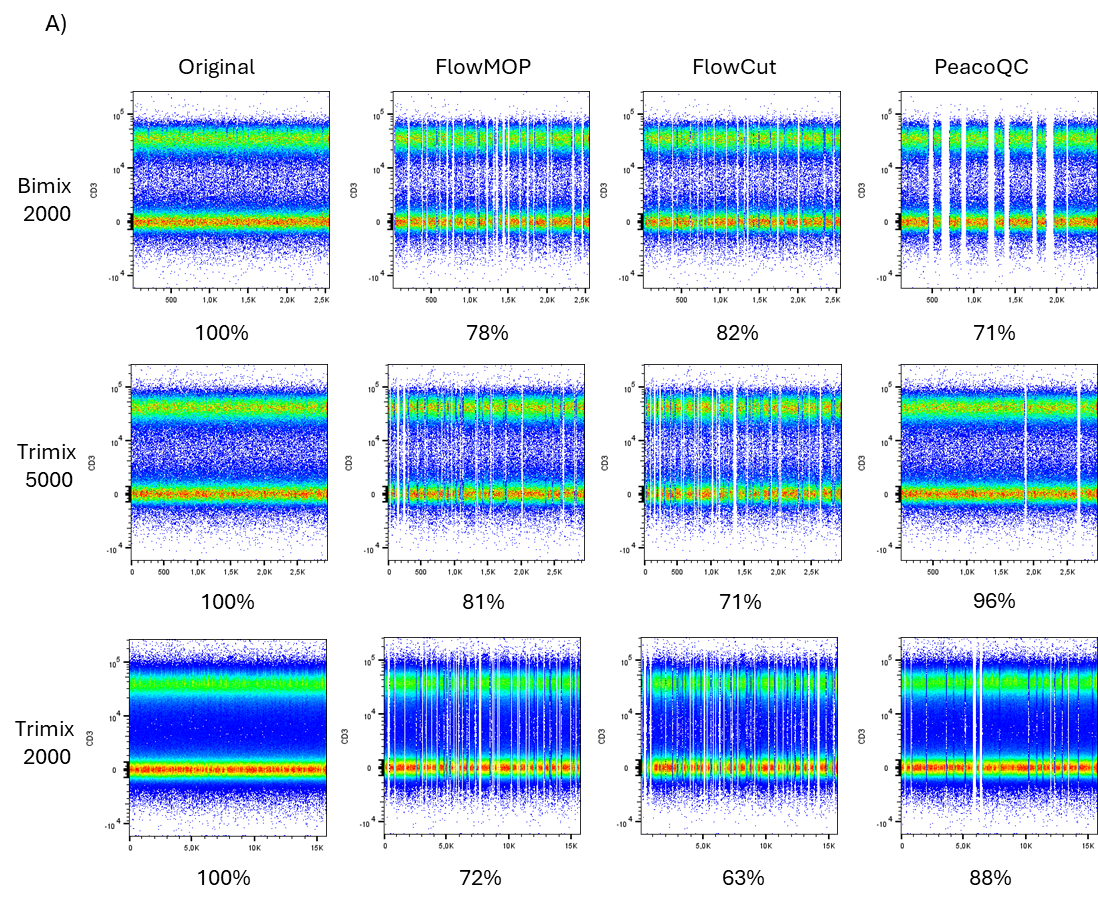
\includegraphics[width=\linewidth,height=0.82\textheight,keepaspectratio]{FlowMOP_submission_media/image8.png}
\begingroup
\renewcommand{\thefigure}{S2}
\caption{Representative flow cytometry CD3 / Time plots for Bimix 2000 bin, Trimix 5000 bin, and Trimix 2000 bin synthetic datasets, with original data inputs, and following cleaning by FlowMOP, FlowCut, and PeacoQC. Percentages below each figure represent the retained proportion of cells relative to the original representative synthetic sample.}
\endgroup
\end{figure}

\begingroup
\small
\setlength{\tabcolsep}{4pt}
\renewcommand{\arraystretch}{1.14}

\captionsetup{type=table}
\begingroup
\renewcommand{\thetable}{S1A}
\captionof{table}{\textbf{Dataset Compositions}}
\endgroup

{\def\LTcaptype{none} % do not increment counter
\begin{longtable}[]{@{}
  >{\raggedright\arraybackslash}p{(\linewidth - 8\tabcolsep) * \real{0.1920}}
  >{\raggedright\arraybackslash}p{(\linewidth - 8\tabcolsep) * \real{0.1920}}
  >{\raggedright\arraybackslash}p{(\linewidth - 8\tabcolsep) * \real{0.1920}}
  >{\raggedright\arraybackslash}p{(\linewidth - 8\tabcolsep) * \real{0.1920}}
  >{\raggedright\arraybackslash}p{(\linewidth - 8\tabcolsep) * \real{0.1920}}@{}}
\toprule\noalign{}
\begin{minipage}[b]{\linewidth}\raggedright
Dataset Name
\end{minipage} & \begin{minipage}[b]{\linewidth}\raggedright
Synthetic Time-Gating Dataset
\end{minipage} & \begin{minipage}[b]{\linewidth}\raggedright
Synthetic Debris-Gating Dataset
\end{minipage} & \begin{minipage}[b]{\linewidth}\raggedright
Synthetic Doublet-Gating Dataset
\end{minipage} & \begin{minipage}[b]{\linewidth}\raggedright
Human Liver
\end{minipage} \\
\midrule\noalign{}
\endhead
\bottomrule\noalign{}
\endlastfoot
Samples (given per benchmarker) & 6, 2 each at 0.5, 1, 3 cell
concentrations, 3 datasets & 4, combined into 3 benchmarking samples &
4, combined into 3 benchmarking samples & 3 \\
Tissue Type & Peripheral blood mononuclear cells & Spleen & Spleen &
Liver tissue \\
Organism & Human & Mouse & Mouse & Human \\
Collection Location & Canberra, ACT, Australia & Canberra, ACT,
Australia & Canberra, ACT, Australia & Sydney, NSW, Australia \\
\end{longtable}
}

\endgroup

\begingroup
\small
\setlength{\tabcolsep}{4pt}
\renewcommand{\arraystretch}{1.14}

\captionsetup{type=table}
\begingroup
\renewcommand{\thetable}{S1A}
\captionof{table}{\textbf{Dataset Compositions} (continued)}
\endgroup

{\def\LTcaptype{none} % do not increment counter
\begin{longtable}[]{@{}
  >{\raggedright\arraybackslash}p{(\linewidth - 8\tabcolsep) * \real{0.1920}}
  >{\raggedright\arraybackslash}p{(\linewidth - 8\tabcolsep) * \real{0.1920}}
  >{\raggedright\arraybackslash}p{(\linewidth - 8\tabcolsep) * \real{0.1920}}
  >{\raggedright\arraybackslash}p{(\linewidth - 8\tabcolsep) * \real{0.1920}}
  >{\raggedright\arraybackslash}p{(\linewidth - 8\tabcolsep) * \real{0.1920}}@{}}
\toprule\noalign{}
\begin{minipage}[b]{\linewidth}\raggedright
Mouse Dorsal Root Ganglion
\end{minipage} & \begin{minipage}[b]{\linewidth}\raggedright
Mouse Skin
\end{minipage} & \begin{minipage}[b]{\linewidth}\raggedright
Mouse Small Intestine
\end{minipage} & \begin{minipage}[b]{\linewidth}\raggedright
Mouse Colon
\end{minipage} & \begin{minipage}[b]{\linewidth}\raggedright
Mouse Brain
\end{minipage} \\
\midrule\noalign{}
\endhead
\bottomrule\noalign{}
\endlastfoot
3 & 3 & 3 & 3 & 4 \\
Dorsal root ganglia & Skin & Distal small intestine & Colon & Brain \\
Mouse & Mouse & Mouse & Mouse & Mouse \\
Canberra, ACT, Australia & Canberra, ACT, Australia & Canberra, ACT,
Australia & Canberra, ACT, Australia & Canberra, ACT, Australia \\
\end{longtable}
}

\endgroup

\begingroup
\small
\setlength{\tabcolsep}{4pt}
\renewcommand{\arraystretch}{1.14}

\captionsetup{type=table}
\begingroup
\renewcommand{\thetable}{S1A}
\captionof{table}{\textbf{Dataset Compositions} (continued)}
\endgroup

{\def\LTcaptype{none} % do not increment counter
\begin{longtable}[]{@{}
  >{\raggedright\arraybackslash}p{(\linewidth - 8\tabcolsep) * \real{0.1920}}
  >{\raggedright\arraybackslash}p{(\linewidth - 8\tabcolsep) * \real{0.1920}}
  >{\raggedright\arraybackslash}p{(\linewidth - 8\tabcolsep) * \real{0.1920}}
  >{\raggedright\arraybackslash}p{(\linewidth - 8\tabcolsep) * \real{0.1920}}
  >{\raggedright\arraybackslash}p{(\linewidth - 8\tabcolsep) * \real{0.1920}}@{}}
\toprule\noalign{}
\begin{minipage}[b]{\linewidth}\raggedright
Mouse Central Nervous System
\end{minipage} & \begin{minipage}[b]{\linewidth}\raggedright
Mouse Spleen
\end{minipage} & \begin{minipage}[b]{\linewidth}\raggedright
Mouse Blood
\end{minipage} & \begin{minipage}[b]{\linewidth}\raggedright
Mouse Bone Marrow
\end{minipage} & \begin{minipage}[b]{\linewidth}\raggedright
Human Cultured T cells
\end{minipage} \\
\midrule\noalign{}
\endhead
\bottomrule\noalign{}
\endlastfoot
3 & 7 & 5 & 3 & 5 \\
Spinal cord and brain & Spleen & Peripherally collected blood & Femur
derived bone marrow & Peripherally collected, cultured, and restimulated
T cells \\
Mouse & Mouse & Mouse & Mouse & Human \\
Canberra, ACT, Australia & Canberra, ACT, Australia & Canberra, ACT,
Australia & Canberra, ACT, Australia & Canberra, ACT, Australia \\
\end{longtable}
}

\endgroup

\begingroup
\small
\setlength{\tabcolsep}{4pt}
\renewcommand{\arraystretch}{1.14}

\captionsetup{type=table}
\begingroup
\renewcommand{\thetable}{S1B}
\captionof{table}{\textbf{Expert / Algorithm IDs}}
\endgroup

{\def\LTcaptype{none} % do not increment counter
\begin{longtable}[]{@{}ll@{}}
\toprule\noalign{}
Expert / Algorithm & ID \\
\midrule\noalign{}
\endhead
\bottomrule\noalign{}
\endlastfoot
Expert 1 & 1 \\
Expert 2 & 2 \\
Expert 3 & 3 \\
Expert 4 & 4 \\
FlowMOP & 5 \\
FlowCut & 6 \\
PeacoQC & 7 \\
\end{longtable}
}

\endgroup

\begingroup
\small
\setlength{\tabcolsep}{4pt}
\renewcommand{\arraystretch}{1.14}

\captionsetup{type=table}
\begingroup
\renewcommand{\thetable}{S1C}
\captionof{table}{\textbf{Time gating rankings (1 = best)}}
\endgroup

{\def\LTcaptype{none} % do not increment counter
\begin{longtable}[]{@{}
  >{\raggedright\arraybackslash}p{(\linewidth - 8\tabcolsep) * \real{0.1920}}
  >{\raggedright\arraybackslash}p{(\linewidth - 8\tabcolsep) * \real{0.1920}}
  >{\raggedright\arraybackslash}p{(\linewidth - 8\tabcolsep) * \real{0.1920}}
  >{\raggedright\arraybackslash}p{(\linewidth - 8\tabcolsep) * \real{0.1920}}
  >{\raggedright\arraybackslash}p{(\linewidth - 8\tabcolsep) * \real{0.1920}}@{}}
\toprule\noalign{}
\begin{minipage}[b]{\linewidth}\raggedright
Rankings
\end{minipage} & \begin{minipage}[b]{\linewidth}\raggedright
Mouse DRG
\end{minipage} & \begin{minipage}[b]{\linewidth}\raggedright
Mouse Skin
\end{minipage} & \begin{minipage}[b]{\linewidth}\raggedright
Human Cultured T Cells
\end{minipage} & \begin{minipage}[b]{\linewidth}\raggedright
Mouse Bone Marrow
\end{minipage} \\
\midrule\noalign{}
\endhead
\bottomrule\noalign{}
\endlastfoot
1 & 3 & 3 & 3 & 3 \\
2 & 1 & 1 & 2 & 5 \\
3 & 4 & 4 & 1 & 4 \\
4 & 2 & 2 & 4 & 1 \\
5 & 5 & 6 & 7 & 2 \\
6 & 6 & 5 & 5 & 6 \\
7 & 7 & 7 & 6 & 7 \\
Mouse Spleen & Mouse Blood & Mouse Brain & Mouse Central Nervous System
& Human Liver \\
3 & 4 & 4 & 1 & 3 \\
4 & 3 & 1 & 4 & 1 \\
1 & 1 & 5 & 3 & 2 \\
7 & 2 & 3 & 2 & 4 \\
5 & 6 & 2 & 5 & 6 \\
6 & 5 & 7 & 7 & 7 \\
2 & 7 & 6 & 6 & 5 \\
\end{longtable}
}

\endgroup

\begingroup
\small
\setlength{\tabcolsep}{4pt}
\renewcommand{\arraystretch}{1.14}

\captionsetup{type=table}
\begingroup
\renewcommand{\thetable}{S1D}
\captionof{table}{\textbf{Debris gating rankings (1 = best)}}
\endgroup

{\def\LTcaptype{none} % do not increment counter
\begin{longtable}[]{@{}
  >{\raggedright\arraybackslash}p{(\linewidth - 8\tabcolsep) * \real{0.1920}}
  >{\raggedright\arraybackslash}p{(\linewidth - 8\tabcolsep) * \real{0.1920}}
  >{\raggedright\arraybackslash}p{(\linewidth - 8\tabcolsep) * \real{0.1920}}
  >{\raggedright\arraybackslash}p{(\linewidth - 8\tabcolsep) * \real{0.1920}}
  >{\raggedright\arraybackslash}p{(\linewidth - 8\tabcolsep) * \real{0.1920}}@{}}
\toprule\noalign{}
\begin{minipage}[b]{\linewidth}\raggedright
Rankings
\end{minipage} & \begin{minipage}[b]{\linewidth}\raggedright
Mouse DRG
\end{minipage} & \begin{minipage}[b]{\linewidth}\raggedright
Mouse Skin
\end{minipage} & \begin{minipage}[b]{\linewidth}\raggedright
Human Cultured T cells
\end{minipage} & \begin{minipage}[b]{\linewidth}\raggedright
Mouse Bone Marrow
\end{minipage} \\
\midrule\noalign{}
\endhead
\bottomrule\noalign{}
\endlastfoot
1 & 3 & 2 & 4 & 3 \\
2 & 2 & 3 & 2 & 2 \\
3 & 1 & 5 & 3 & 1 \\
4 & 4 & 4 & 1 & 4 \\
5 & 5 & 1 & 5 & 5 \\
Mouse Spleen & Mouse Blood & Mouse Brain & Mouse Central Nervous System
& Human Liver \\
3 & 5 & 3 & 3 & 2 \\
2 & 3 & 2 & 2 & 1 \\
1 & 2 & 4 & 4 & 5 \\
4 & 4 & 1 & 5 & 3 \\
5 & 1 & 5 & 1 & \\
\end{longtable}
}

\endgroup

\begingroup
\small
\setlength{\tabcolsep}{4pt}
\renewcommand{\arraystretch}{1.14}

\captionsetup{type=table}
\begingroup
\renewcommand{\thetable}{S1E}
\captionof{table}{\textbf{Doublet gating rankings (1 = best)}}
\endgroup

{\def\LTcaptype{none} % do not increment counter
\begin{longtable}[]{@{}
  >{\raggedright\arraybackslash}p{(\linewidth - 8\tabcolsep) * \real{0.1920}}
  >{\raggedright\arraybackslash}p{(\linewidth - 8\tabcolsep) * \real{0.1920}}
  >{\raggedright\arraybackslash}p{(\linewidth - 8\tabcolsep) * \real{0.1920}}
  >{\raggedright\arraybackslash}p{(\linewidth - 8\tabcolsep) * \real{0.1920}}
  >{\raggedright\arraybackslash}p{(\linewidth - 8\tabcolsep) * \real{0.1920}}@{}}
\toprule\noalign{}
\begin{minipage}[b]{\linewidth}\raggedright
Rankings
\end{minipage} & \begin{minipage}[b]{\linewidth}\raggedright
Mouse DRG
\end{minipage} & \begin{minipage}[b]{\linewidth}\raggedright
Mouse Skin
\end{minipage} & \begin{minipage}[b]{\linewidth}\raggedright
Human Cultured T cells
\end{minipage} & \begin{minipage}[b]{\linewidth}\raggedright
Mouse Bone Marrow
\end{minipage} \\
\midrule\noalign{}
\endhead
\bottomrule\noalign{}
\endlastfoot
1 & 2 & 2 & 1 & 4 \\
2 & 3 & 3 & 4 & 2 \\
3 & 1 & 1 & 3 & 1 \\
4 & 5 & 5 & 2 & 5 \\
5 & 4 & 4 & 5 & \\
Mouse Spleen & Mouse Blood & Mouse Brain & Mouse Central Nervous System
& Human Liver \\
3 & 3 & 3 & 4 & 3 \\
4 & 2 & 1 & 3 & 5 \\
1 & 1 & 4 & 1 & 2 \\
5 & 5 & 5 & 2 & 4 \\
2 & 4 & 2 & 5 & 1 \\
\end{longtable}
}

\endgroup

\begingroup
\small
\setlength{\tabcolsep}{4pt}
\renewcommand{\arraystretch}{1.14}

\captionsetup{type=table}
\begingroup
\renewcommand{\thetable}{S2}
\captionof{table}{\textbf{Jeffreys' Scale}}
\endgroup

{\def\LTcaptype{none} % do not increment counter
\begin{longtable}[]{@{}ll@{}}
\toprule\noalign{}
Bayes Factor & Hypothesis descriptor \\
\midrule\noalign{}
\endhead
\bottomrule\noalign{}
\endlastfoot
\textless1 & Null hypothesis supported \\
1-3 & Anecdotal / Weak evidence \\
3-10 & Moderate / Substantial evidence \\
10-30 & Very strong evidence \\
\textgreater30 & Decisive evidence \\
\end{longtable}
}

\endgroup

\clearpage
\begin{landscape}
\begingroup
\scriptsize
\setlength{\tabcolsep}{3pt}
\renewcommand{\arraystretch}{1.12}

\captionsetup{type=table}
\begingroup
\renewcommand{\thetable}{S3A}
\captionof{table}{\textbf{Retention and permissiveness-adjusted Zombie-high exclusion following combined time, debris, and doublet filtering in human liver samples}}
\endgroup

{\def\LTcaptype{none} % do not increment counter
\begin{longtable}[]{@{}
  >{\raggedright\arraybackslash}p{(\linewidth - 20\tabcolsep) * \real{0.0873}}
  >{\raggedright\arraybackslash}p{(\linewidth - 20\tabcolsep) * \real{0.0873}}
  >{\raggedleft\arraybackslash}p{(\linewidth - 20\tabcolsep) * \real{0.0873}}
  >{\raggedleft\arraybackslash}p{(\linewidth - 20\tabcolsep) * \real{0.0873}}
  >{\raggedleft\arraybackslash}p{(\linewidth - 20\tabcolsep) * \real{0.0873}}
  >{\raggedleft\arraybackslash}p{(\linewidth - 20\tabcolsep) * \real{0.0873}}
  >{\raggedleft\arraybackslash}p{(\linewidth - 20\tabcolsep) * \real{0.0873}}
  >{\raggedleft\arraybackslash}p{(\linewidth - 20\tabcolsep) * \real{0.0873}}
  >{\raggedleft\arraybackslash}p{(\linewidth - 20\tabcolsep) * \real{0.0873}}
  >{\raggedleft\arraybackslash}p{(\linewidth - 20\tabcolsep) * \real{0.0873}}
  >{\raggedleft\arraybackslash}p{(\linewidth - 20\tabcolsep) * \real{0.0873}}@{}}
\toprule\noalign{}
\begin{minipage}[b]{\linewidth}\raggedright
Sample
\end{minipage} & \begin{minipage}[b]{\linewidth}\raggedright
Tissue
\end{minipage} & \begin{minipage}[b]{\linewidth}\raggedleft
Manual retained (\%)
\end{minipage} & \begin{minipage}[b]{\linewidth}\raggedleft
FlowMOP retained (\%)
\end{minipage} & \begin{minipage}[b]{\linewidth}\raggedleft
Zombie-high in raw (\%)
\end{minipage} & \begin{minipage}[b]{\linewidth}\raggedleft
Zombie-high among FlowMOP-removed (\%)
\end{minipage} & \begin{minipage}[b]{\linewidth}\raggedleft
Zombie-low removed (\%)
\end{minipage} & \begin{minipage}[b]{\linewidth}\raggedleft
Zombie-high removed (\%)
\end{minipage} & \begin{minipage}[b]{\linewidth}\raggedleft
Manual selectivity ratio
\end{minipage} & \begin{minipage}[b]{\linewidth}\raggedleft
FlowMOP selectivity ratio
\end{minipage} & \begin{minipage}[b]{\linewidth}\raggedleft
FlowMOP/manual fold-change
\end{minipage} \\
\midrule\noalign{}
\endhead
\bottomrule\noalign{}
\endlastfoot
LB180 & Non-tumour & 58.1 & 64.1 & 17.2 & 27.9 & 31.3 & 58.0 & 1.13 &
1.85 & 1.64 \\
LB192 & Non-tumour & 74.0 & 79.1 & 1.4 & 4.1 & 20.3 & 61.5 & 1.12 & 3.03
& 2.70 \\
LB200 & Non-tumour & 31.3 & 53.7 & 9.2 & 17.3 & 42.2 & 86.9 & 1.17 &
2.06 & 1.76 \\
LB202 & Tumour & 37.9 & 62.0 & 55.4 & 64.8 & 30.0 & 44.4 & 0.86 & 1.48 &
1.71 \\
LB236 & Tumour & 38.6 & 54.1 & 64.7 & 54.4 & 59.3 & 38.5 & 0.74 & 0.65 &
0.88 \\
LB262 & Tumour & 68.0 & 53.6 & 21.6 & 29.8 & 41.5 & 63.9 & 1.88 & 1.54 &
0.82 \\
Summary & Six samples & 51.3 ± 17.8 & 61.1 ± 10.0 & & & & & 1.13 median
& 1.70 median & 1.68 median (0.82-2.70) \\
\end{longtable}
}

\endgroup
\end{landscape}
\clearpage

Selectivity is the Zombie-high removal rate divided by the Zombie-low
removal rate. The primary exact two-sided paired Wilcoxon signed-rank
test was applied to log-transformed FlowMOP/manual selectivity ratios (p
= 0.156). FlowMOP output is the intersection of the time, debris, and
doublet masks and excludes the limit-of-detection mask. Zombie-low was
defined operationally as Zombie UV-A \textless12,000 raw units. Manual
populations were reconstructed from the FlowJo workspace.

\begingroup
\small
\setlength{\tabcolsep}{4pt}
\renewcommand{\arraystretch}{1.14}

\captionsetup{type=table}
\begingroup
\renewcommand{\thetable}{S3B}
\captionof{table}{\textbf{Constituent FlowMOP gate selectivity}}
\endgroup

{\def\LTcaptype{none} % do not increment counter
\begin{longtable}[]{@{}
  >{\raggedright\arraybackslash}p{(\linewidth - 8\tabcolsep) * \real{0.1920}}
  >{\raggedleft\arraybackslash}p{(\linewidth - 8\tabcolsep) * \real{0.1920}}
  >{\raggedleft\arraybackslash}p{(\linewidth - 8\tabcolsep) * \real{0.1920}}
  >{\raggedleft\arraybackslash}p{(\linewidth - 8\tabcolsep) * \real{0.1920}}
  >{\raggedleft\arraybackslash}p{(\linewidth - 8\tabcolsep) * \real{0.1920}}@{}}
\toprule\noalign{}
\begin{minipage}[b]{\linewidth}\raggedright
Sample
\end{minipage} & \begin{minipage}[b]{\linewidth}\raggedleft
Time
\end{minipage} & \begin{minipage}[b]{\linewidth}\raggedleft
Debris
\end{minipage} & \begin{minipage}[b]{\linewidth}\raggedleft
Doublet
\end{minipage} & \begin{minipage}[b]{\linewidth}\raggedleft
Combined
\end{minipage} \\
\midrule\noalign{}
\endhead
\bottomrule\noalign{}
\endlastfoot
LB180 & 1.08 & 1.46 & 4.89 & 1.85 \\
LB192 & 1.04 & N/A & 5.64 & 3.03 \\
LB200 & 1.27 & 0.02 & 9.13 & 2.06 \\
LB202 & 0.95 & 0.10 & 60.85 & 1.48 \\
LB236 & 0.97 & 0.15 & 246.30 & 0.65 \\
LB262 & 1.04 & 1.34 & 4.77 & 1.54 \\
Median & 1.04 & 0.15 & 7.38 & 1.70 \\
\end{longtable}
}

\endgroup

Values are Zombie-high/Zombie-low removal-rate ratios; values above 1
indicate preferential Zombie-high exclusion. The LB192 debris ratio is
undefined because the debris mask removed no events. The extreme LB202
and LB236 doublet ratios reflect near-zero removal of Zombie-low events.

\begingroup
\small
\setlength{\tabcolsep}{4pt}
\renewcommand{\arraystretch}{1.14}

\captionsetup{type=table}
\begingroup
\renewcommand{\thetable}{S4}
\captionof{table}{\textbf{Full-dataset FlowMOP MAD-smoothing analysis}}
\endgroup

{\def\LTcaptype{none} % do not increment counter
\begin{longtable}[]{@{}lrrr@{}}
\toprule\noalign{}
Short, long smoothing factors & Sensitivity & Specificity & Balanced
mean \\
\midrule\noalign{}
\endhead
\bottomrule\noalign{}
\endlastfoot
\texttt{0,0} (no-smoothing control) & 0.8021 & \textbf{0.7081} &
\textbf{0.75506} \\
\textbf{\texttt{0.01,0.05} (current default)} & 0.8212 & 0.6811 &
\textbf{0.75114} \\
\texttt{0.02,0.05} & 0.8228 & 0.6794 & 0.75108 \\
\texttt{0.01,0.02} & 0.8112 & 0.6885 & 0.74986 \\
\texttt{0.02,0.09} & \textbf{0.8276} & 0.6709 & 0.74923 \\
\texttt{0.01,0.09} & 0.8257 & 0.6707 & 0.74823 \\
\texttt{0.05,0.09} & 0.8188 & 0.6676 & 0.74317 \\
\texttt{0.02,0.20} & 0.8248 & 0.6479 & 0.73632 \\
\texttt{0.05,0.20} & 0.8197 & 0.6520 & 0.73586 \\
\texttt{0.01,0.20} & 0.8231 & 0.6477 & 0.73540 \\
\texttt{0.10,0.20} & 0.8138 & 0.6415 & 0.72769 \\
\texttt{0.05,0.34} & 0.8194 & 0.6344 & 0.72686 \\
\texttt{0.02,0.34} & 0.8199 & 0.6286 & 0.72424 \\
\texttt{0.10,0.34} & 0.8134 & 0.6250 & 0.71921 \\
\texttt{0.10,0.50} & 0.8139 & 0.6229 & 0.71842 \\
\texttt{0.10,0.90} (former default) & 0.8139 & 0.6226 & 0.71827 \\
\texttt{0.10,1.00} & 0.8139 & 0.6226 & 0.71827 \\
\texttt{0.20,0.90} & 0.8007 & 0.6142 & 0.70747 \\
\texttt{0.40,0.90} & 0.7812 & 0.6140 & 0.69756 \\
\end{longtable}
}

\endgroup

Values are equally weighted macro-averages across the six Figure 2
benchmark groups (173 primary inputs; six tied-composition inputs
excluded). The balanced mean is the arithmetic mean of sensitivity and
specificity. Bold indicates the highest value overall and the highest
balanced mean among smoothed settings.

\begin{figure}[p]
\centering
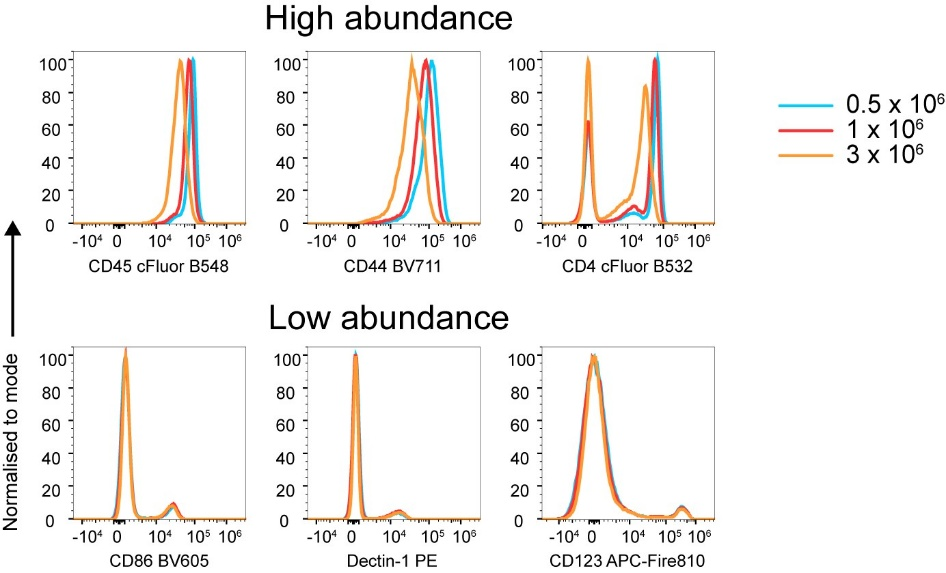
\includegraphics[width=\linewidth,height=0.82\textheight,keepaspectratio]{FlowMOP_submission_media/image9.jpeg}
\begingroup
\renewcommand{\thefigure}{S3}
\caption{Fluorescence variation as a function of cell concentration.}
\endgroup
\end{figure}

\begin{figure}[p]
\centering
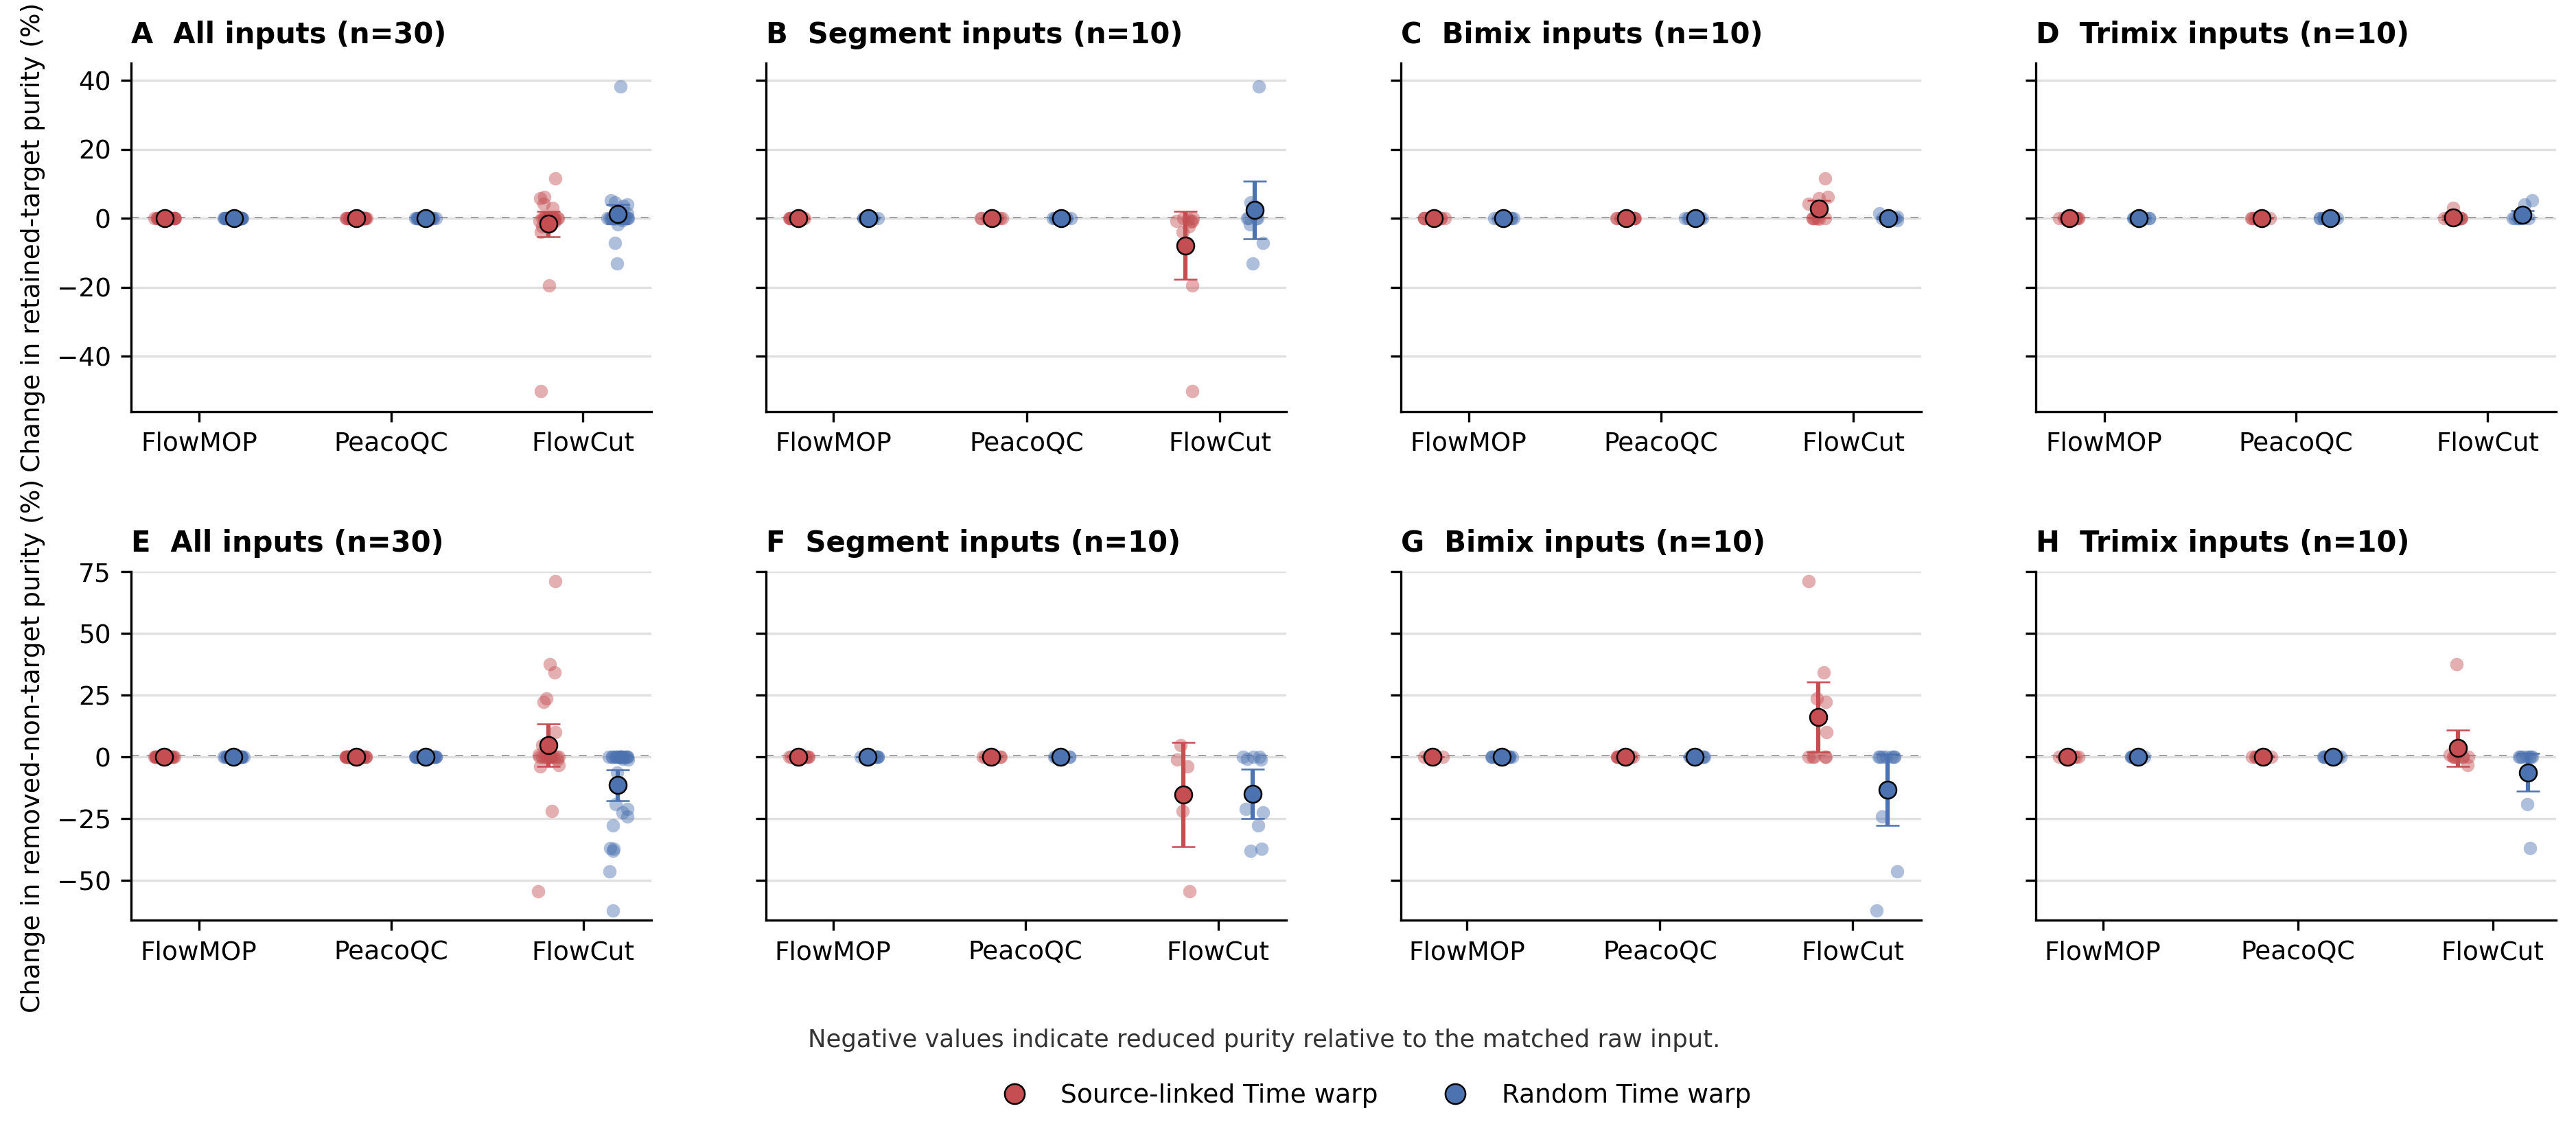
\includegraphics[width=\linewidth,height=0.82\textheight,keepaspectratio]{figs_data/revision_timewarp_mechanism.png}
\begingroup
\renewcommand{\thefigure}{S4}
\caption{Time-only acquisition-rate perturbations reveal FlowCut sensitivity to local Time density. Points show raw-matched changes in sensitivity and specificity, with large points and intervals showing the mean and 95\% confidence interval. Negative values indicate reduced performance relative to the raw control. Columns show all inputs together and the Segment, Bimix, and Trimix subsets separately. FlowMOP and PeacoQC remain unchanged under both source-linked and random Time warping. In contrast, FlowCut\textquotesingle s sensitivity and specificity shift after Time-only perturbation, with the clearest specificity loss in random Time-warped inputs and the strongest source-linked sensitivity loss in Segment inputs, where acquisition-rate structure aligns with source composition.}
\endgroup
\end{figure}

\subsection{Supplementary expert preference
evaluation}\label{supplementary-expert-preference-evaluation}

The expert-ranking exercise was performed using gates generated with an
earlier FlowMOP configuration. It is therefore retained as an
exploratory historical evaluation rather than a primary assessment of
the current selected implementation. The rankings measure relative
preference and do not establish absolute gating adequacy or event-level
accuracy.

\subsubsection{Supplementary methods}\label{supplementary-methods}

The expert-ranking analysis was used to summarize relative preferences
among gates generated by FlowMOP, comparator algorithms, and human
operators; it was not treated as an absolute measure of gating adequacy.

Rankings were modelled using a Plackett--Luce model with latent method
abilities; identifiability was enforced by fixing a reference ability to
zero. Independent Normal priors were placed on non-reference abilities.
Posterior inference was performed with an affine-invariant ensemble
Markov Chain Monte Carlo sampler (emcee; 32 walkers, 5,000 iterations;
1,000 burn-in), and posterior medians with 95\% credible intervals were
reported. Directional hypotheses (superiority/inferiority) were
evaluated by computing P = Pr(H1 \textbar{} data) and converting to a
Bayes factor BF$_{10}$ = p/(1 -- p) under equal prior odds, interpreted
using Jeffreys' scale and reported as BF, P (Bayes factor, posterior
probability of the alternative hypothesis) (Table S2).

For each Plackett--Luce fit, the ensemble sampler's mean acceptance
fraction and an integrated-autocorrelation-time-based effective sample
size were monitored (both as implemented in emcee) to assess MCMC
convergence. Across all analyses, mean acceptance fractions ranged from
0.520 to 0.60, and effective sample sizes ranged from 128,003 to
134,042.

Posterior predictive checks compared observed pairwise win counts with
those implied by posterior draws under a Bradley--Terry formulation,
using a chi-square-type discrepancy averaged over method pairs. The
maximum average χ² per comparison was 0.56, indicating good agreement
between the model and the observed rankings.

Computations were implemented in Python with numerically stable
log-likelihoods.

\subsubsection{Supplementary results}\label{supplementary-results}

FlowMOP outputs were compared with expert-provided gates using a
forced-ranking preference task across nine biological datasets. These
rankings measure relative expert preference and should not be
interpreted as an absolute measure of gating adequacy. The resulting
time, debris, and doublet gates were ranked by an expert familiar with
that sample type. FlowCut and PeacoQC were also included in the
time-gating comparison. Rank 1 indicates greatest preference.

\begin{figure}[p]
\centering
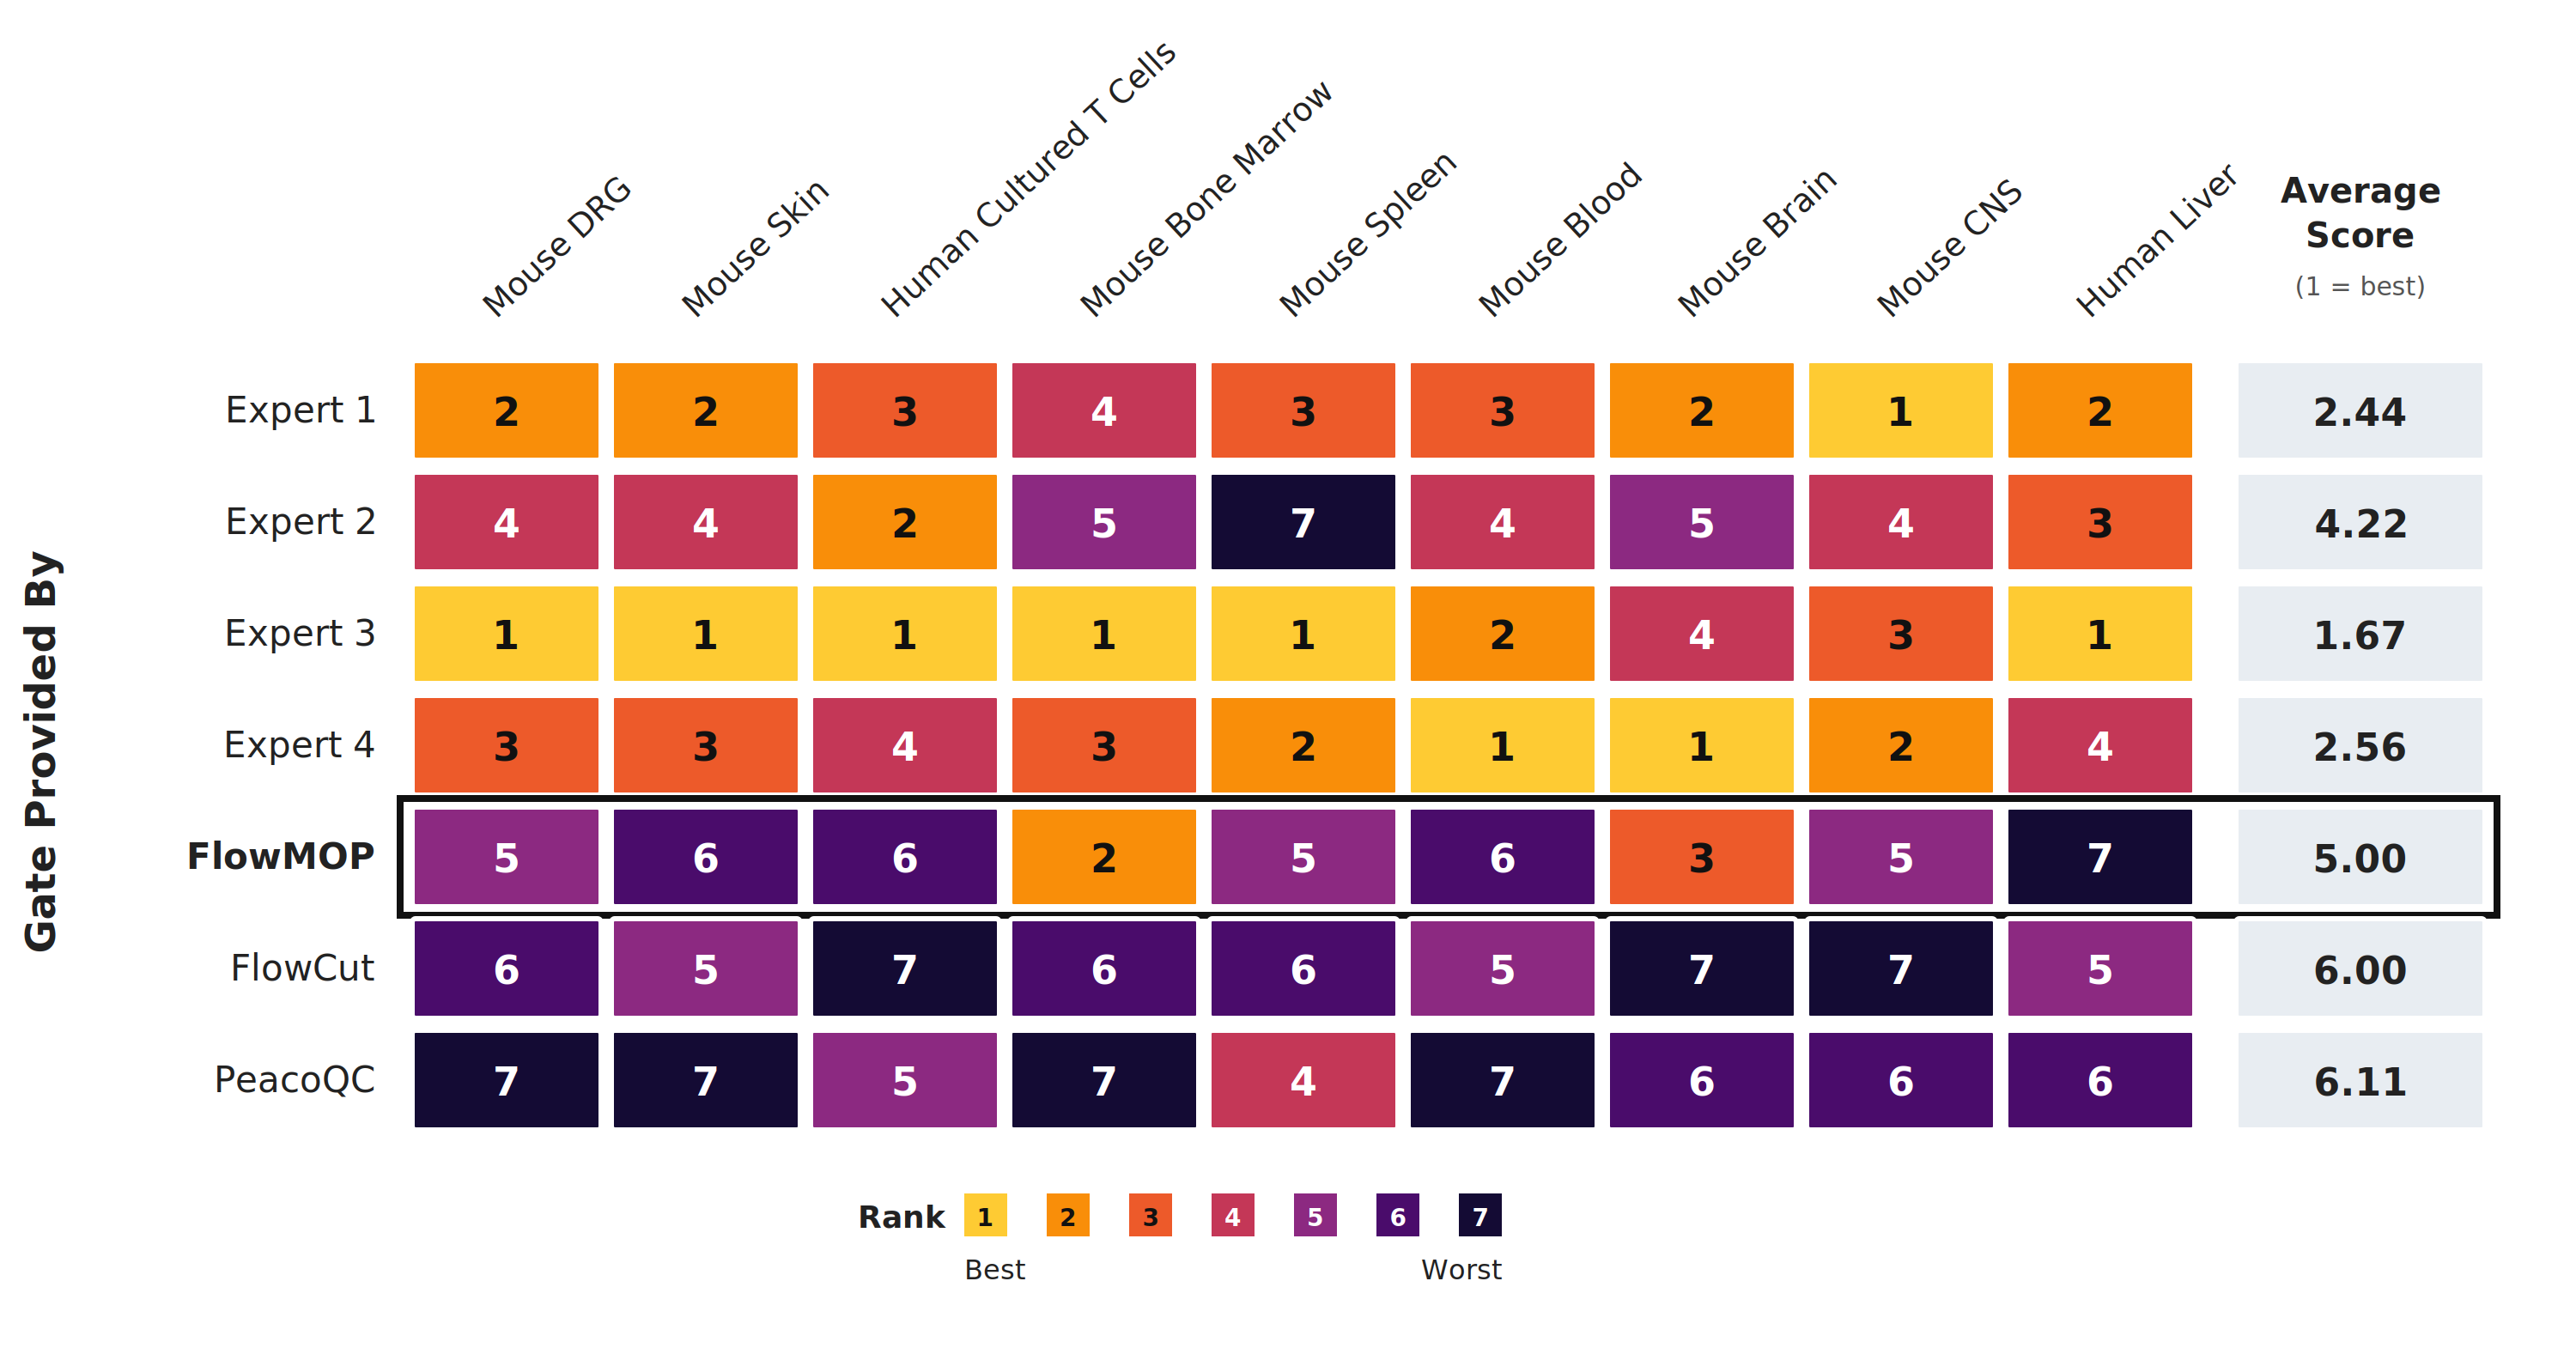
\includegraphics[width=\linewidth,height=0.82\textheight,keepaspectratio]{FlowMOP_submission_media/image5_revised.png}
\begingroup
\renewcommand{\thefigure}{S5}
\caption{Expert preference rankings for time gates provided by four human experts, FlowMOP (black border), FlowCut, and PeacoQC across nine datasets. Rows indicate the gate provider, and the final column shows the mean rank across datasets. Rank 1 indicates greatest preference; therefore, a lower average score indicates greater preference. Abbreviations: DRG, dorsal root ganglion; CNS, central nervous system.}
\endgroup
\end{figure}

In the biological datasets, FlowMOP had the lowest mean rank among the
algorithmic time-gating approaches (Fig. S5). In the mouse brain and
mouse bone marrow tasks, it ranked third and second, respectively (Fig.
S5). On a Bayesian analysis, FlowMOP was observed to be substantially
preferred to FlowCut (BF = 5.39, P = 84.3\%) and strongly preferred to
PeacoQC (BF = 12.10, P = 92.4\%). FlowMOP was ranked inferiorly to all
human experts with strong to decisive evidence (Expert 2 BF = 10.55, P =
91.3\%, all others BF \textgreater{} 100, P = 100\%).

\begin{figure}[p]
\centering
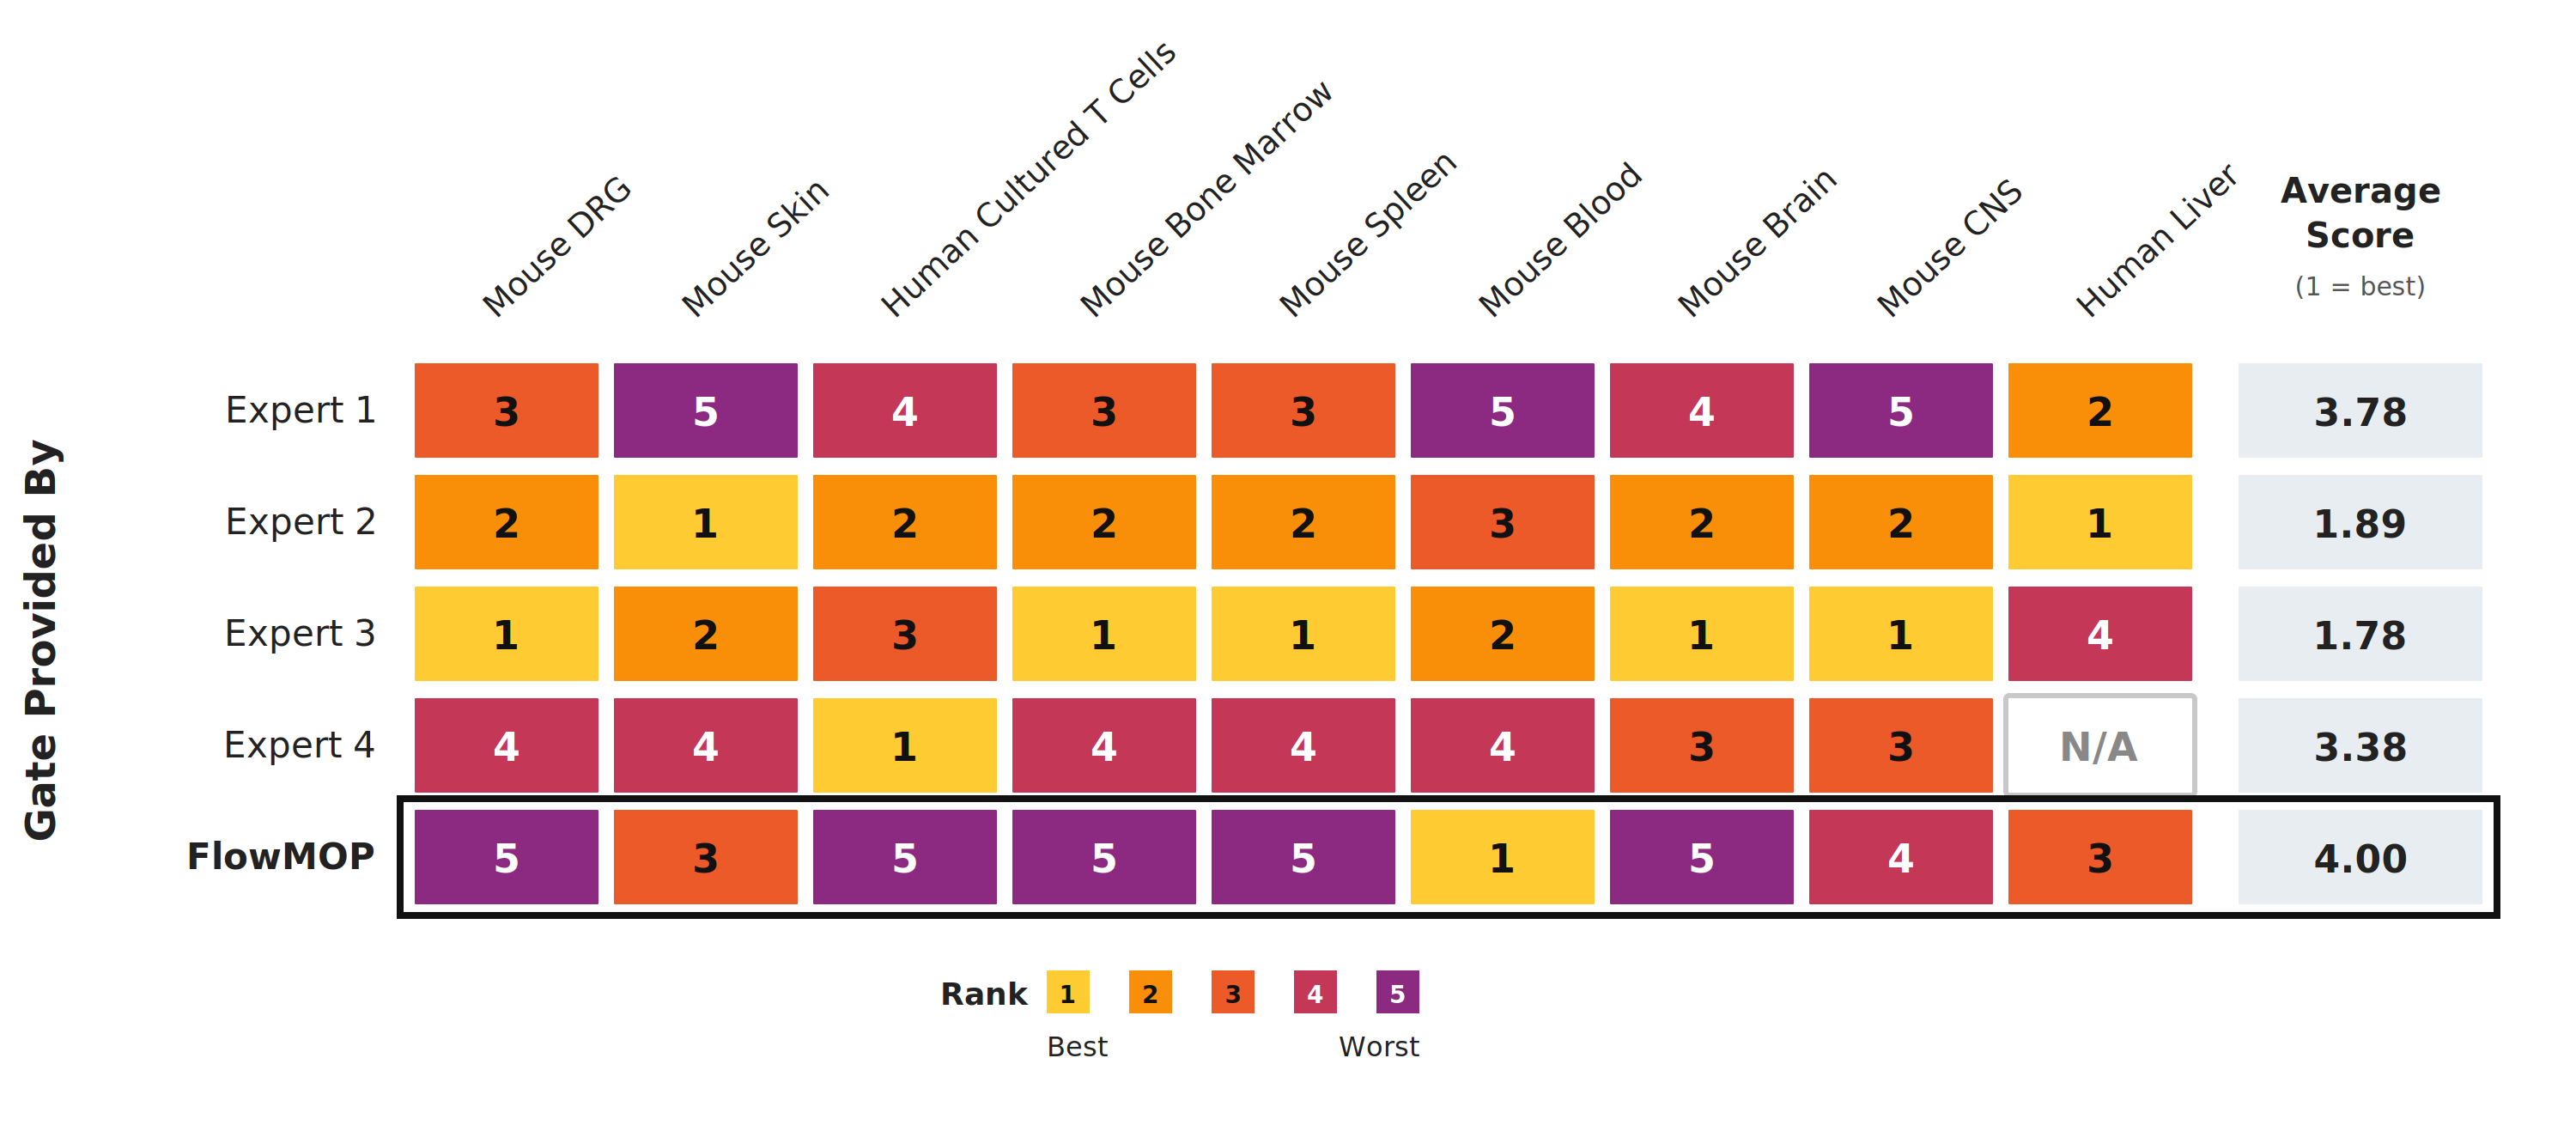
\includegraphics[width=\linewidth,height=0.82\textheight,keepaspectratio]{FlowMOP_submission_media/image6_revised.png}
\begingroup
\renewcommand{\thefigure}{S6}
\caption{Expert preference rankings for debris gates provided by four human experts and FlowMOP (black border) across nine datasets. Rows indicate the gate provider, and the final column shows the mean rank across available datasets. Rank 1 indicates greatest preference; therefore, a lower average score indicates greater preference. N/A denotes an unavailable gate.}
\endgroup
\end{figure}

\begin{figure}[p]
\centering
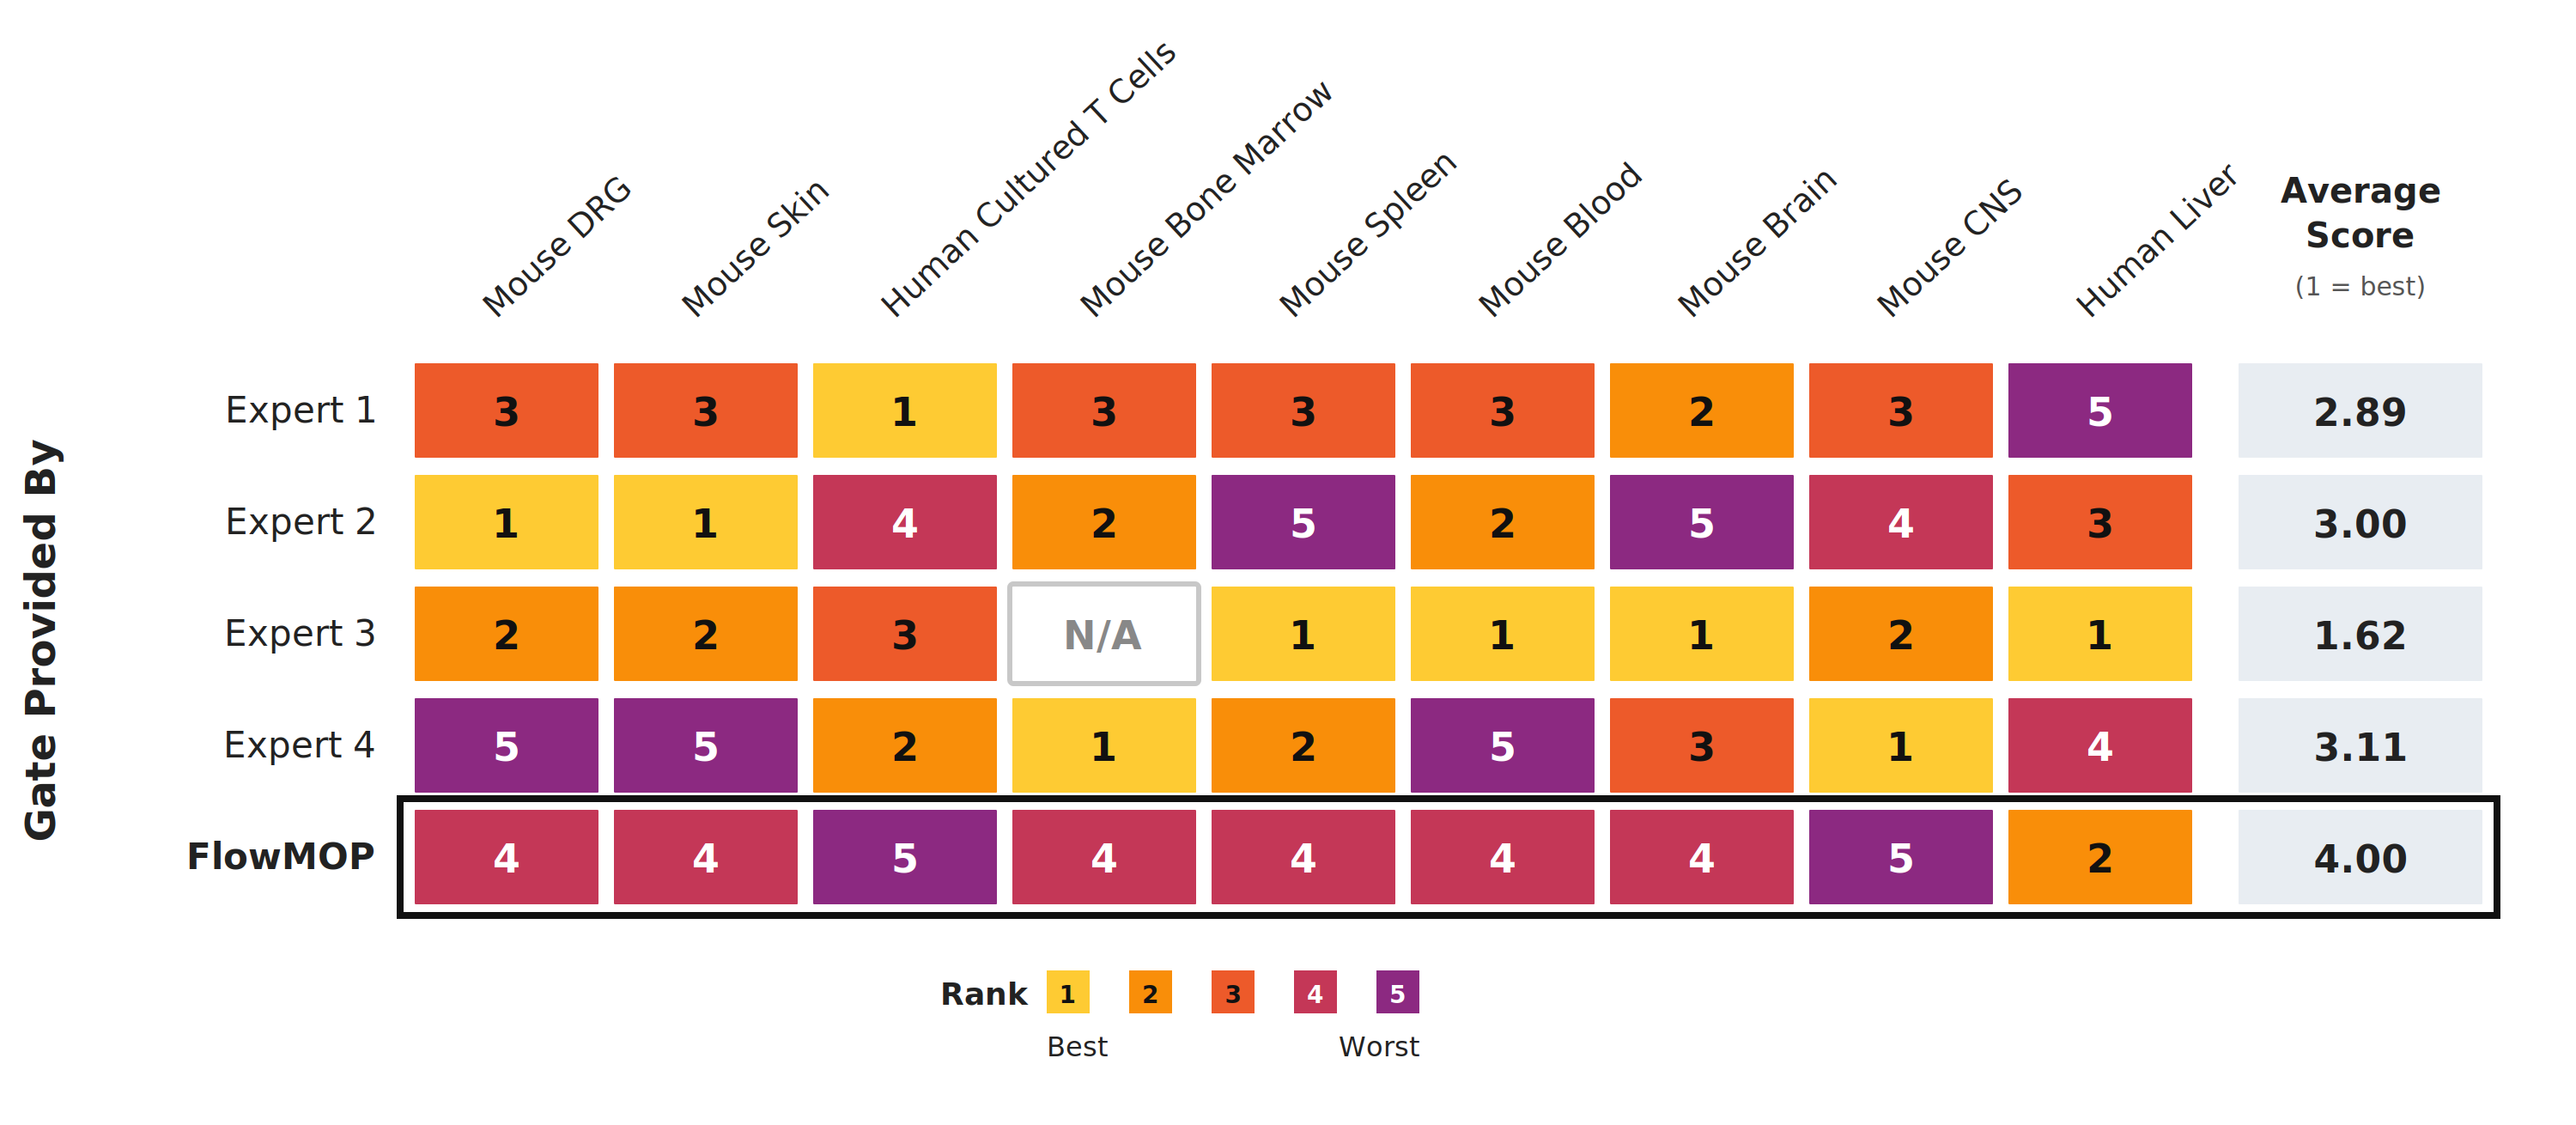
\includegraphics[width=\linewidth,height=0.82\textheight,keepaspectratio]{FlowMOP_submission_media/image7_revised.png}
\begingroup
\renewcommand{\thefigure}{S7}
\caption{Expert preference rankings for doublet gates provided by four human experts and FlowMOP (black border) across nine datasets. Rows indicate the gate provider, and the final column shows the mean rank across available datasets. Rank 1 indicates greatest preference; therefore, a lower average score indicates greater preference. N/A denotes an unavailable gate.}
\endgroup
\end{figure}

FlowMOP had the highest mean rank when compared with the human experts
for debris and doublet removal (Figs. S6, S7). On a Bayesian analysis,
substantial to strong evidence was observed for FlowMOP being inferior
to Expert 1 (BF = 5.87, P = 85.5\%), Expert 4 (BF = 12.85, P = 92.8\%),
and Experts 2 and 3 (BF \textgreater{} 100, P = 100\%) in debris
removal. In doublet removal, FlowMOP was weakly inferiorly ranked to
Expert 4 (BF = 3.14, P = 75.8\%), substantially inferiorly ranked to
Expert 1 (BF = 5.67, P = 85.0\%), strongly inferiorly ranked to Expert 2
(BF = 14.38, P = 93.5\%), and decisively inferiorly ranked to Expert 3
(BF \textgreater{} 100, P = 100\%).

FlowMOP's relative expert preference varied across datasets. For debris,
it ranked first in the mouse blood task and third in the human liver and
mouse skin datasets. In the doublet task, FlowMOP ranked second in the
human liver task. Full tabular rankings are provided in Tables S1B-E.

\FloatBarrier

\clearpage

\section{References}\label{references}

\begin{hangparas}{1.5em}{1}

{[}1{]} Aysun Adan, Günel Alizada, Yağmur Kiraz, Yusuf Baran, and Ayten
Nalbant. 2017. Flow cytometry: basic principles and applications.
Critical Reviews in Biotechnology 37, 2 (February 2017), 163--176.
\url{https://doi.org/10.3109/07388551.2015.1128876}

{[}2{]} Thomas Myles Ashhurst, Felix Marsh-Wakefield, Givanna Haryono
Putri, Alanna Gabrielle Spiteri, Diana Shinko, Mark Norman Read, Adrian
Lloyd Smith, and Nicholas Jonathan Cole King. 2022. Integration,
exploration, and analysis of high-dimensional single-cell cytometry data
using Spectre. Cytometry Part A 101, 3 (2022), 237--253.
\url{https://doi.org/10.1002/cyto.a.24350}

{[}3{]} Noah Castelo, Maarten W. Bos, and Donald R. Lehmann. 2019.
Task-Dependent Algorithm Aversion. Journal of Marketing Research 56, 5
(October 2019), 809--825. \url{https://doi.org/10.1177/0022243719851788}

{[}4{]} Antonio Cosma. 2020. The Nightmare of a Single Cell: Being a
Doublet. Cytometry A 97, 8 (August 2020), 768--771.
\url{https://doi.org/10.1002/cyto.a.23929}

{[}5{]} Annelies Emmaneel, Katrien Quintelier, Dorine Sichien, Paulina
Rybakowska, Concepción Marañón, Marta E. Alarcón-Riquelme, Gert Van
Isterdael, Sofie Van Gassen, and Yvan Saeys. 2022. PeacoQC: Peak-based
selection of high quality cytometry data. Cytometry Part A 101, 4
(2022), 325--338. \url{https://doi.org/10.1002/cyto.a.24501}

{[}6{]} Kipper Fletez-Brant, Josef Špidlen, Ryan R. Brinkman, Mario
Roederer, and Pratip K. Chattopadhyay. 2016. flowClean: Automated
identification and removal of fluorescence anomalies in flow cytometry
data. Cytometry Part A 89, 5 (2016), 461--471.
\url{https://doi.org/10.1002/cyto.a.22837}

{[}7{]} Zicheng Hu, Alice Tang, Jaiveer Singh, Sanchita Bhattacharya,
and Atul J. Butte. 2020. A robust and interpretable end-to-end deep
learning model for cytometry data. Proceedings of the National Academy
of Sciences 117, 35 (September 2020), 21373--21380.
\url{https://doi.org/10.1073/pnas.2003026117}

{[}8{]} Nanditha Mallesh. 2023. Automated analysis of flow cytometry
using deep learning for the detection of B-cell neoplasms. Thesis.
Universitäts- und Landesbibliothek Bonn. Retrieved August 7, 2023 from
\url{https://bonndoc.ulb.uni-bonn.de/xmlui/handle/20.500.11811/10949}

{[}9{]} Justin Meskas, Daniel Yokosawa, Sherrie Wang, Gabriela C. Segat,
and Ryan Remy Brinkman. 2023. FlowCut: An R package for automated
removal of outlier events and flagging of files based on time versus
fluorescence analysis. Cytometry Part A 103, 1 (2023), 71--81.
\url{https://doi.org/10.1002/cyto.a.24670}

{[}10{]} Gianni Monaco, Hao Chen, Michael Poidinger, Jinmiao Chen, João
Pedro de Magalhães, and Anis Larbi. 2016. flowAI: automatic and
interactive anomaly discerning tools for flow cytometry data.
Bioinformatics 32, 16 (August 2016), 2473--2480.
\url{https://doi.org/10.1093/bioinformatics/btw191}

{[}11{]} Christina Bligaard Pedersen, Søren Helweg Dam, Mike Bogetofte
Barnkob, Michael D. Leipold, Noelia Purroy, Laura Z. Rassenti, Thomas J.
Kipps, Jennifer Nguyen, James Arthur Lederer, Satyen Harish Gohil,
Catherine J. Wu, and Lars Rønn Olsen. 2022. cyCombine allows for robust
integration of single-cell cytometry datasets within and across
technologies. Nat Commun 13, 1 (March 2022), 1698.
\url{https://doi.org/10.1038/s41467-022-29383-5}

{[}12{]} Lisa Weijler, Florian Kowarsch, Michael Reiter, Pedro
Hermosilla, Margarita Maurer-Granofszky, and Michael Dworzak. 2024.
FATE: Feature-Agnostic Transformer-Based Encoder for Learning
Generalized Embedding Spaces in Flow Cytometry Data. 2024. 7956--7964.
Retrieved May 3, 2024 from
\url{https://openaccess.thecvf.com/content/WACV2024/html/Weijler_FATE_Feature-Agnostic_Transformer-Based_Encoder_for_Learning_Generalized_Embedding_Spaces_in_WACV_2024_paper.html}

{[}13{]} Kenneth Lo, Ryan Remy Brinkman, and Raphael Gottardo. 2008.
Automated gating of flow cytometry data via robust model-based
clustering. Cytometry Part A 73A, 4 (April 2008), 321--332.
\url{https://doi.org/10.1002/cyto.a.20531}

{[}14{]} Lukas Fisch, Michael Heming, Andreas Schulte-Mecklenbeck,
Catharina C. Gross, Stefan Zumdick, Carlotta Barkhau, Daniel Emden, Jan
Ernsting, Ramona Leenings, Kelvin Sarink, Nils R. Winter, Udo
Dannlowski, Heinz Wiendl, Gerd Meyer zu Hörste, and Tim Hahn. 2024.
GateNet: A novel neural network architecture for automated flow
cytometry gating. Computers in Biology and Medicine 179 (September
2024), 108820. \url{https://doi.org/10.1016/j.compbiomed.2024.108820}

{[}15{]} Jiong Chen, Matei Ionita, Yanbo Feng, Yinfeng Lu, Patryk
Orzechowski, Sumita Garai, Kenneth Hassinger, Jingxuan Bao, Junhao Wen,
Duy Duong-Tran, Joost Wagenaar, Michelle L. McKeague, Mark M. Painter,
Divij Mathew, Ajinkya Pattekar, Nuala J. Meyer, E. John Wherry, Allison
R. Greenplate, and Li Shen. 2025. Automated cytometric gating with
human-level performance using bivariate segmentation. Nature
Communications 16, 1 (February 2025), 1576.
\url{https://doi.org/10.1038/s41467-025-56622-2}

{[}16{]} Chris P. Verschoor, Alina Lelic, Jonathan L. Bramson, and Dawn
M. E. Bowdish. 2015. An introduction to automated flow cytometry gating
tools and their implementation. Frontiers in Immunology 6 (July 2015),
380. \url{https://doi.org/10.3389/fimmu.2015.00380}

\end{hangparas}

\end{document}
